
% to choose your degree
% please un-comment just one of the following
\documentclass[bsc,frontabs,twoside,singlespacing,parskip,deptreport]{infthesis}     % for BSc, BEng etc.
% \documentclass[minf,frontabs,twoside,singlespacing,parskip,deptreport]{infthesis}  % for MInf
\usepackage[utf8]{inputenc}
\usepackage{epigraph}
\usepackage{graphicx} %Added by Songbo
\usepackage{multirow}
\usepackage{rotating} %Added by Songbo
\usepackage{lscape} %Added by Songbo
\usepackage{booktabs}
\usepackage{longtable}
\usepackage{tabu}
\usepackage{amsthm}
\usepackage{color}
\usepackage{gb4e}
\usepackage{pdfpages}
\usepackage{attachfile2}

\usepackage{etoolbox}% http://ctan.org/pkg/etoolbox


% Flexible Qoute
\usepackage{epigraph,varwidth}

\usepackage{pifont}% http://ctan.org/pkg/pifont

\usepackage{amssymb}




\newcommand{\bluecheck}{{\color{blue}\checkmark}}
\newcommand{\xmark}{\color{red}\ding{55}}%


\newtheorem{observation}{Observation}[chapter]
\newtheorem{hypo}{Hypothesis}[chapter]

\newbool{insubexample}
\newtheorem{example}{Example}[section]% Example
\newtheorem{subexample}{Example}[example]% Sub-example
\renewcommand{\thesubexample}{\theexample(\alph{subexample})}%
\AtBeginEnvironment{example}{\global\boolfalse{insubexample}}%
\AtBeginEnvironment{subexample}{%
  \ifbool{insubexample}{}{\global\booltrue{insubexample}%
    \refstepcounter{example}}%
}%







\renewcommand{\epigraphsize}{\small}
\setlength{\epigraphwidth}{0.6\textwidth}
\renewcommand{\textflush}{flushright}
\renewcommand{\sourceflush}{flushright}
% A useful addition
\newcommand{\epitextfont}{\itshape}
\newcommand{\episourcefont}{\scshape}


\makeatletter
\newsavebox{\epi@textbox}
\newsavebox{\epi@sourcebox}
\newlength\epi@finalwidth
\renewcommand{\epigraph}[2]{%
  \vspace{\beforeepigraphskip}
  {\epigraphsize\begin{\epigraphflush}
   \epi@finalwidth=\z@
   \sbox\epi@textbox{%
     \varwidth{\epigraphwidth}
     \begin{\textflush}\epitextfont#1\end{\textflush}
     \endvarwidth
   }%
   \epi@finalwidth=\wd\epi@textbox
   \sbox\epi@sourcebox{%
     \varwidth{\epigraphwidth}
     \begin{\sourceflush}\episourcefont#2\end{\sourceflush}%
     \endvarwidth
   }%
   \ifdim\wd\epi@sourcebox>\epi@finalwidth 
     \epi@finalwidth=\wd\epi@sourcebox
   \fi
   \leavevmode\vbox{
     \hb@xt@\epi@finalwidth{\hfil\box\epi@textbox}
     \vskip1.75ex
     \hrule height \epigraphrule
     \vskip.75ex
     \hb@xt@\epi@finalwidth{\hfil\box\epi@sourcebox}
   }%
   \end{\epigraphflush}
   \vspace{\afterepigraphskip}}}
\makeatother

% End Flexiable Qoute


\begin{document}



\title{Building Coherent Open-domain Dialogue Systems: Data Collection and Analysis}

\author{Songbo Hu}

% to choose your course
% please un-comment just one of the following
\course{Artificial Intelligence and Computer Science}
%\course{Artificial Intelligence and Software Engineering}
%\course{Artificial Intelligence and Mathematics}
%\course{Artificial Intelligence and Psychology }   
%\course{Artificial Intelligence with Psychology }   
%\course{Linguistics and Artificial Intelligence}    
%\course{Computer Science}
%\course{Software Engineering}
%\course{Computer Science and Electronics}    
%\course{Electronics and Software Engineering}    
%\course{Computer Science and Management Science}    
%\course{Computer Science and Mathematics}
%\course{Computer Science and Physics}  
%\course{Computer Science and Statistics}    

% to choose your report type
% please un-comment just one of the following
%\project{Undergraduate Dissertation} % CS&E, E&SE, AI&L
%\project{Undergraduate Thesis} % AI%Psy
\project{4th Year Project Report}

\date{\today}

\abstract{

Recent advances in neural network based language models enable us to learn entire dialogue models directly from conversational data. However, most of the previous systems have failed to model the longer prior context of the conversation adequately, thereby creating a situation where extended dialogues rapidly become incoherent and unnatural sounding. There is no existing dialogue corpus which contains natural conversations and is able to provide strong supervision signals to train dialogue systems with reinforcement learning. In this project, we design and collect a novel corpus contains extended coherent dialogues of questions and responses that are information in a knowledge graph. These dialogues describe the relations within a knowledge graph with clear links between the phrases in the questions to nodes in a knowledge graph. The purpose for this corpus is to perform statistical analysis about various linguistic patterns within coherent dialogues, thereby, create a framework for neural models to learn how to parse these patterns and produce more coherent responses. We mainly focus on investigating when the appearance of an elided construction is natural and convey the intended content. A detailed statistical analysis have been conducted to support our investigation.
}

\maketitle

\section*{Acknowledgements}

This thesis is the result of my undergraduate journey. Many people have influenced, inspired and supported me during the journey. First and foremost, I would like to thank my supervisor Prof. Alex Lascarides for providing guidance, feedback and constant help for this project. Her mentorship has not just greatly influenced my work on this thesis, but will influence my research career. I am enormously grateful to all the staff at the University of Edinburgh, my personal tutor Prof. Jane Hillston, all my lecturers, ITO, Advice Place... They offer constant support and make me stronger during my journey. Special thanks goes to Informatics Student Services, who have funded this project and make the creation of our corpus possible. I appreciate all the help from whom I had to share this journey with, my lovely participants in this project, my friends and my colleges at Edinburgh. Last, but certainly not least, I would like to thank to my family in China for their selfless support and encouragement, without whom, my journey would never start at the beginning.


\tableofcontents

%\pagenumbering{arabic}

\chapter{Introduction}

\epigraph{When was Alan Turing born? \\
Alan Turing was born on Sunday 13 June 1912. \\
Where was he born? \\
Alan Turing was born in Warrington Lodge. \\
Who is his father? \\
Julius Mathison Turing is Alan Turing's father.\\
When was he born? \\
Julius Mathison Turing was born 9 November 1873. \\
Where? \\
You're at Edinburgh, Scotland.
}{\textit{Songbo and Siri 2020}}

A dialogue system is a conversational agent that can converse with humans in natural language. It can help us solve many tedious tasks effectively or bring entertainment value to our daily life. Recent advances in dialogue systems (such as virtual assistants\cite{alexa,cortana,siri}) enable us to engage in natural conversational interactions and access to machine readable knowledge and information with computers. It substantially increases the accessibility of state of the art technologies to people with diverse backgrounds. And for those with impairments, it could transform their daily living into a journey toward capability instead of disability.

Since Alan Turing published his landmark work in 1950\cite{turing1950computing}, the intelligence level of a machine is described as how well the machine is able to fool a human into believing that it, the machine, is a human based on its text responses. If a human is unable to distinguish the difference between the machine from a human, the machine is said to have passed the Turing test. We could say such a machine signifies a significantly high level of intelligence. It has been the goal for the development of dialogue systems for decades and various attempts have been proposed to pass the Turing test. Recently, advances in neural network based language models enable us to learn entire dialogue models directly from conversational data. Although we improve the performance of neural models by increasing the number of parameters and training with more data, we are still far from our goal. Most of the previous systems have failed to model the longer prior context of the conversation adequately, thereby creating a situation where extended dialogues rapidly become incoherent and unnatural sounding, with repetition being a key problem. 

\begin{exe}
	\ex
		\begin{xlist}
			\ex \label{q1} Q: When was Alan Turing born?
			\ex \label{a1} A: Alan Turing was born on Sunday 13 June 1912.
			\ex \label{q2} Q: Where was he born?
			\ex \label{a2} A: Alan Turing was born in Warrington Lodge.
			\ex \label{q3} Q: Who is his father?
			\ex \label{a3} A: Julius Mathison Turing is Alan Turing’s father.
			\ex \label{q4} Q: When was he born?
			\ex \label{a4} A: Julius Mathison Turing was born 9 November 1873.
			\ex \label{q5} Q: Where?
			\ex \label{a5} A: You’re at Edinburgh, Scotland.
	\end{xlist}
	\end{exe}

As I demonstrated in the example conversation at the beginning of the chapter and repeated here, humans tend to utilise linguistic patterns, such as anaphora and sluicing to reduce repetitions. For example, in the human utterance \ref{q2}, human uses pronoun "he" to refer "Alan Turing" in question \ref{a1}. This is a typical example use of anaphora, which leads to a more concise sentence. In addition, human utterance \ref{q5} is an example of sluicing construction. Information, which can be inferred from the context, is omitted. A more refined definition of these linguistics patterns is provided in our Annotation Schema in Appendix \ref{appendix:annotation}.

In contrast, dialogue systems rarely produces pronouns and unable to model elided construction therefore produce unnatural speech in the context. For example, in order to answer the second question \ref{q2}, humans are able to interpret the anaphora (He refers to Alan Turing.) and produce a short answer (In Warrington Lodge.). Compared to human's responses, Siri's responses \ref{a2} are heavy and verbose. The challenge for Siri, and many other dialogue systems, is to know when such an answer conveys the intended content, and when it doesn't. The system has to make a decent decision on when content can be elided while still ensuring that the user can easily interpret the system's message and retrieve that message accurately. In addition, a wrong interpretation of a question could lead to an unhelpful and diverged response. Siri fails to understand the context to parse fragments and interpret the sluicing in the final question \ref{q5}. The misunderstanding of the context leads to a completely unhelpful and incoherent response \ref{a5}. The main reasons of this unnaturalness for Siri is the lack of reliable systematic analysis of such linguistic patterns and the inadequate representation of the context. It is a problem which need to be adequately addressed before our agents could look forward to attempting the Turing test.

We aim to address the gap in our understanding of the interaction between topic shifts on the one hand and the natural use of anaphora and elided constructions on the other by designing and implementing a method of data collection of humans engaged in question answering in extended dialogue, where we control the way the topic shifts in the course of a conversation. The resulting data provides an opportunity to systematically analyse the effects of topic shifts on the decisions that competent human language users make on whether to use anaphora and/or elided constructions. We motivate and describe the way we collected data in Chapter 3 and present an analysis of the data collected in Chapter 4.

In this section, we will briefly review the recent development of dialogue systems. Specifically, we will discuss two types of dialogue systems: the chit-chat dialogue systems (known as chatbots), and the task-oriented dialogue systems. We will focus on machine learning approaches to developing such systems, rather than the use of hand-crafted rules, since the former methods are now dominant and the latter are highly brittle and restricted to toy domains. We will discuss their architectures, pros and cons, and their main limitations to achieve coherent open-domain conversations. The majority of this thesis is about how to create an environment for neural models to learn linguistic patterns within coherent extended dialogues and how to integrate these models into the existing dialogue systems. It constitutes a first step towards modelling coherent open-domain conversations and will potentially enable the existing dialogue systems utilising valuable linguistic information to produce coherent responses.

\section {A Brief Review of Existing Dialogue Systems}

\subsection{The Chit-chat Dialogue System}

The chit-chat dialogue systems are usually called chatbots. These systems are designed and implemented to carry extended conversations with the goal of mimicking the ‘chats’ characteristic of informal human-human interaction\cite{jurafsky2019speech}. They are mainly aiming to provide entertainment value. Existing chatbots majorly fall into the following subcategories: the rule-based systems, the corpus-based systems, as will be discussed in order below.

\subsubsection*{The Rule-based Systems}

Instead of letting machines learn the conversation strategy from human behaviours, which we could encode directly as rules. Dialogue agents could use these rules to generate dialogue utterances effectively. Normally, a message input will be processed by a set of carefully pre-defined rules e.g., a key-word look-up dictionary, if-else conditions, or more sophisticated machine learning classifiers\cite{jiweilithesis}. Consequently, the dialogue agent would produce a natural language response by outputting an utterance in storage, manipulating the input message or selecting some related historical contexts based on these rules.

\begin{figure}[h]
    \centering
    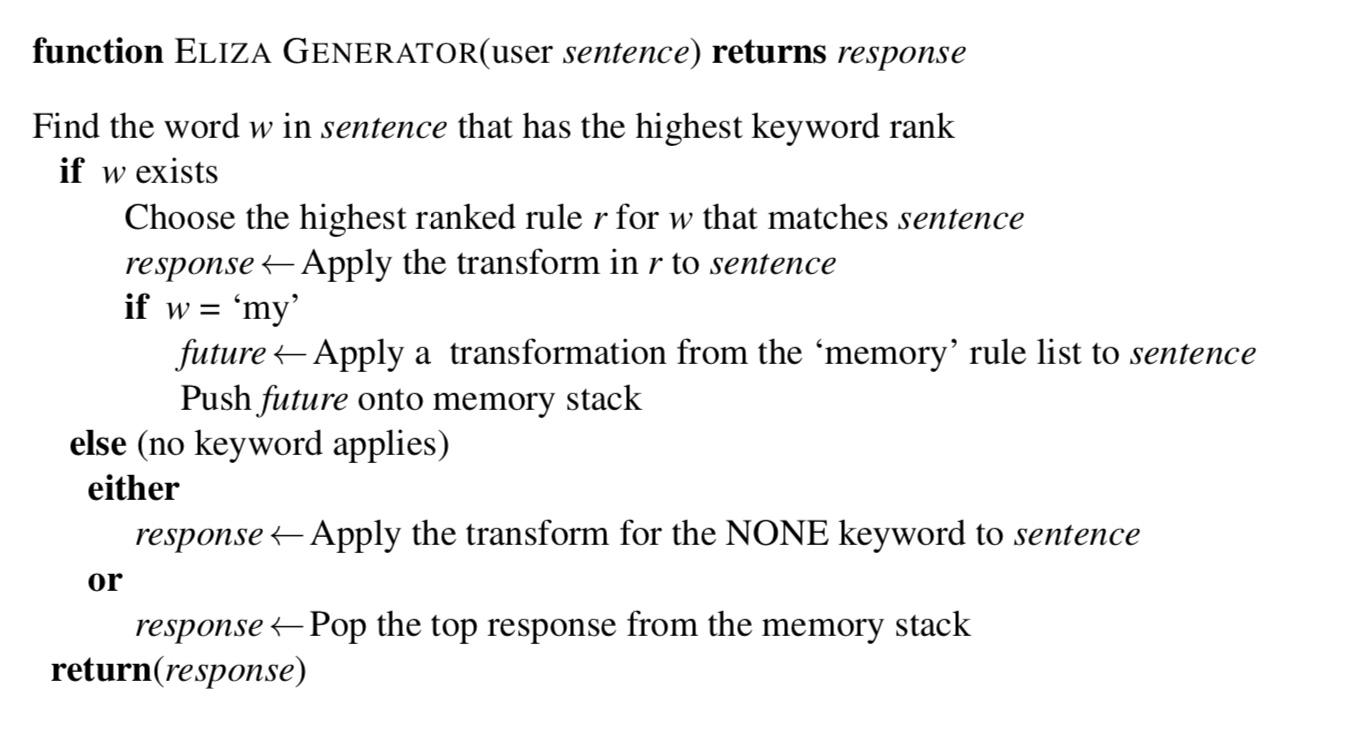
\includegraphics[width=0.9\textwidth]{elizarule.jpeg}
    \caption{A simplified sketch of the ELIZA algorithm.}
    \label{fig:elizarule}
\end{figure}

There are many well-known rule-based dialogue systems in history, such as ELIZA\cite{weizenbaum1966eliza} \footnote{It is instructive that the purpose of building Eliza was to show that it is sometimes possible to fake understanding via hand-crafted rules based on key word search and template generation, even though there is no interpretation component or parsing in the system at all.}, SHRDLU\cite{winograd1972shrdlu}, ALICE\cite{wallace1995artificial}. There are also languages such as Artificial Intelligence Markup Language(AIML), which provides an effect tool to write sophisticated conversations logic in a machine-readable format\cite{wallace1995artificial}.

The development of rule-based systems is an important milestone in developing modern dialogue systems. Many of them are very sophisticated and well engineered, which they attempted to model dialogue in an explanatory and deep way. The architecture of such a system involves the whole pipeline of natural language processing. However, their drawbacks are obvious: rule-based systems predominantly rely on the set of pre-defined rules and these rules have to be carefully designed and implemented. Building a sophisticated rule-based system is very expensive because the number of these rules escalates rapidly. Rule-based systems do not have the ability to understand human languages and generate meaningful natural language utterances\cite{jiweilithesis}. Consequently, they are very brittle and only able to conduct very superficial conversations. Despite the lack of intelligence, even with the recent rapid development of large fancy neural network architecture and increasing number of conversational corpora, these rule-based dialogue systems could always provide a very strong baseline.

\subsubsection*{The Corpus-based Systems}

Coding conversation logics manually is astronomically expensive and infeasible for many applications. Corpus-based dialogue system could potentially alleviate this issue by mining human-human conversations, or sometimes mining the human responses from human-machine conversations, instead of using hand-built rules. These data-driven approaches are becoming widely popular due to the increasing computing power and the creation of large scale conversational dataset. 

There are two common architectures for such system: information retrieval (IR), and machine learned sequence transduction. Due to the limitation that IR-based chatbots can only mirror training data, it is often to treat response generation as a machine translation task which transduces from the user’s prior turn to the system’s turn. This method offers the promise of scalability and language-independence, together with the capacity to capture contextual dependencies in a way not possible with IR-based approaches.

\begin{figure}[h]
    \centering
    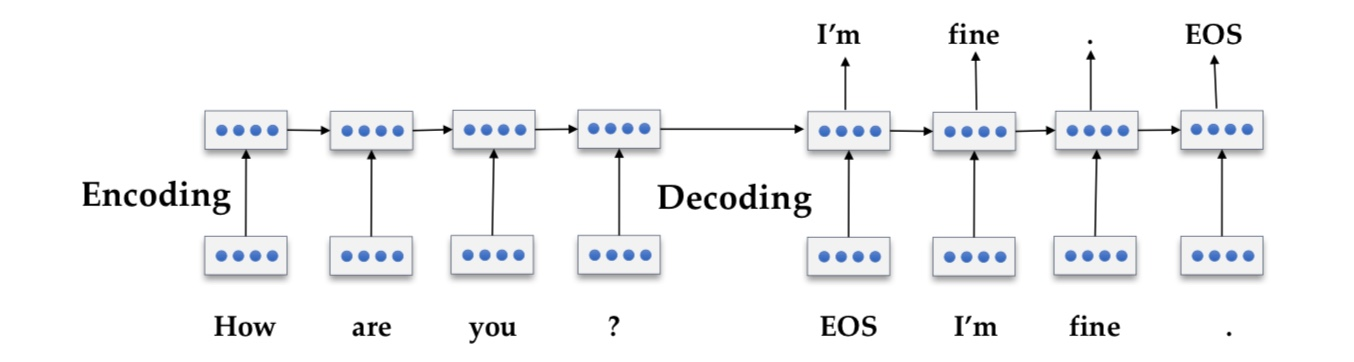
\includegraphics[width=0.9\textwidth]{seq2seq.jpeg}
    \caption{A sequence to sequence model for neural response generation.\cite{jurafsky2019speech}}
    \label{fig:seq2seq}
\end{figure}

This idea was firstly developed by Ritter et al\cite{ritter2011data}. (cited in Jurafsky and Martin\cite{jurafsky2019speech}) using phrase-based machine translation to translate a user turn to a system response. In 2015, transduction models for response generation were modelled using encoder-decoder (seq2seq) models\cite{shang2015neural,strub2017end,sordoni2015neural}. However, the simple seq2seq generation architecture is unable to model the prior context of the conversation. Serban et al\cite{serban2016building} suggests a hierarchical (HRED) model that summarizes information over multiple prior turns. This model consists of two recurrent neural networks (RNNs) stacked on top of each other: one is a sentence-level RNN which encodes each utterance into a fixed length vector, while a conversation-level RNN takes each utterance vector as input and outputs a vector that summarizes the conversation so far. The vector is mapped back to text using a recurrent decoder. This gives a way for the previous information to be passed to future turns as hidden states\cite{lowe2017training}.

\begin{figure}[h]
    \centering
    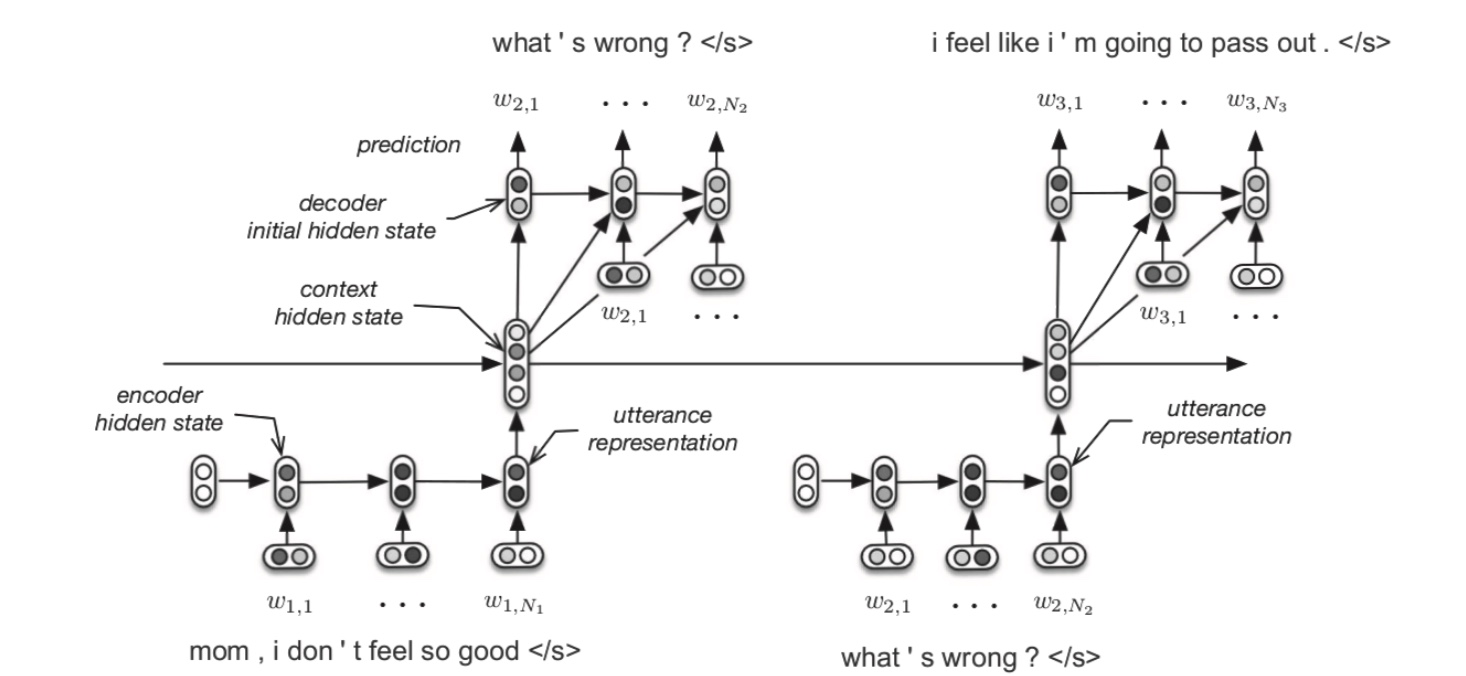
\includegraphics[width=0.9\textwidth]{HERD.jpeg}
    \caption{The computational graph of the HRED architecture for a dialogue composed of three turns.}
    \label{fig:HERD}
\end{figure}

However, even if one has access to an enormous dataset for training, there is still a significant proportion of unseen dialogue states. Techniques, such as smoothing, can only help to a limited extent, because of the radical extent to which data is sparse. Consequently, generating responses using end-to-end methods tends to generate generic, uninformative and non-coherent replies (e.g., generating ``I don’t know." regardless of the context). In addition, encoder-decoder response generators focus on generating single responses, instead of forming a coherent continuous conversation\cite{jurafsky2019speech}. Humans could easily notice these unnatural and mechanical responses (e.g. the Siri conversation above). Techniques, such as Reinforcement learning (RL)\cite{li2016deep} and adversarial networks\cite{li2017adversarial}, can be used to address this issue.

\subsection{The Goal-oriented Dialogue System}

 Goal-oriented dialogue systems are sometimes also called task-based dialogue systems, in which they converse with users to help complete tasks like making a restaurant reservation, booking a hotel or setting up an alarm. Famous examples of such agents are digital assistants (Siri, Alexa, Google Home, Cortana, et.)\cite{siri,alexa,googlehome,cortana} which can be viewed as a combination of chatbots and goal-oriented dialogue systems. With the power of cloud computing and internet of things technologies, these conversations AIs are changing our daily life and developing a 10 billion pounds worth industry\cite{chatbotmarket}. Here, I would like to introduce the architectures of existing statistical spoken dialogue systems (hereafter SDSs) and their main challenges to perform coherent conversations in an open domain. 

\begin{figure}[h]
    \centering
    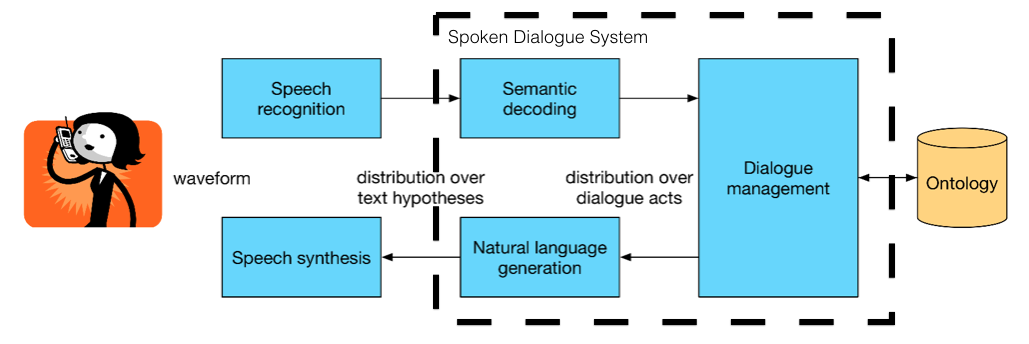
\includegraphics[width=0.80\textwidth]{sds.png}
    \caption{Architecture of a Spoken Dialogue System.\cite{gasic}}
    \label{fig:sds}
\end{figure}

Current SDSs have three key components which are shown as Figure\ref{fig:sds}. A semantics decoder decodes the meaning in utterances into dialogue acts which describe the current intention of the user, for example, confirm(food=Korean). Then, a dialogue manager, which usually consists of a belief tracker and a policy network, will keep track of the belief states and produce a dialogue act as the response. The dialogue manager treats dialogue generation as a partially observable Markov decision process (POMDP)\cite{williams2007partially,young2013pomdp,young2010hidden} which explicitly models the uncertainty natural of human conversations with Bayesian methods. Such framework provides robustness against the errors created by the speech recognition. Later a semantic encoder (natural language generator) will map this act back into a natural language response.

However, keeping track of the belief states under such a framework presents a tough challenge. Exact model representation is infeasible due to the limitation of computational complexity\cite{young2013pomdp}. Carefully constructed approximation and additional independent assumption are needed. For example, if we are willing to find an expensive 5-star hotel in the city center, in order to make the inference practical, we have to assume that there is no relation between a hotel is expensive and it is a 5-star hotel. It is clearly not true. In addition, as shown in Figure \ref{fig:sds}, pre-defined ontology is needed in order to keep track of the dialogue state. This makes the existing dialogue system infeasible to perform conversations in an open-domain. One research direction would be building a SDS which can support a natural conversation about any topic within a wide coverage Knowledge Graph (KG). This forms the definition of an open-domain spoken dialogue system\cite{opendomain}.




\section {Thesis Outline}

In this thesis, we mainly focus on creating a framework in which neural models could learn linguistic patterns within extended coherent dialogues.

Firstly, we explore how to build such a framework by designing, collecting and annotating a conversational dataset. This dataset consists of extended coherent dialogues of questions and responses. These dialogues should describe the relations within a knowledge graph with clear links between the phrases in the questions to nodes in a knowledge graph. Secondly, we analyse the collected dataset statistically in order to investigate how human behave differently under different context in different domain. Later, we will introduce a proposed neural model to model these linguistic patterns and how the existing dialogue systems could benefit from this model.

We start off by providing background knowledge on available corpora to train dialogue models and how to evaluate these dialogue models in Chapter 2. In Chapter 3 and Chapter 4, we will describe the design and creation of our framework in details and perform analysis to figure out the common patterns within these dialogues. Chapter 5 will introduce our proposed neural models and methods in order to model coherent dialogues with neural networks. We will briefly summarize our findings and mention some further work in Chapter 6.

\chapter{Background}

In this chapter, we investigate the existing resources and frameworks to build a neural dialogue model and summarize the popular evaluation metrics for the dialogue modeling task.

\section{Corpora for Training Dialogue Models}

Humans perform dialogues with different purposes, under different situations and in different medias. There is a vast amount of data available documenting human communications. Some of these data is collected as corpora and these corpora can be classified into different categories. Each category has different characteristics, utilities and applications. In order to make the most of the available resources, we discuss the important distinctions between each type of dialogue corpora: whether the corpus features constrained or unconstrained dialogues; whether a corpus is written, spoken; whether a corpus features human-human interactions or human-machine interactions. Afterwards, I give a brief summary about current public available corpora.

\subsection{Chit-chat or Goal-oriented Corpora}

People use different languages for different purposes. We may want to call an airliner to book a ticket or chat with our friends to share our brilliant ideas. The purpose and motivation of our conversation will have a significant influence on the language we use. Similarly, the way in which a dialogue corpus is collected can also have a significant influence on the model we built from. Some conversations are relatively causal, informal and unconstrained, which we usually call them chit-chats. There are many chit-chat corpora and most of them are aiming to mimic spontaneous and unplanned spoken interactions between humans. Consequently, they are also referred as Spontaneous (Unconstrained) Corpora\cite{serban2018survey}. Another large proportion of the existing corpora focus on a particular topic or intend to solve a specific task. In such situations, the task or topic is pre-specified and participants are discouraged from deviating from the topic. We refer to these as Task-Oriented or Constrained Dialogue Corpora.

Dialogues in spontaneous corpora usually have richer grammar and vocabularies, which reflect our daily communication well. However, such corpora are usually in plain text with less informative annotations. Consequently, people usually train models with end-to-end methods using those corpora. Such setting could reduce the interpretability of models' reasoning and pose additional challenges to models' evaluation, which we will discuss in later section. 

For constrained dialogues, some experimental conditions in which dialogues were collected can result in unnatural behaviours. Consequently, dialogues in goal-oriented corpora usually don't bear a close resemblance to our daily communication and do not correlate well to the true typical dialogue patterns in natural conversations. Therefore, all experimental conditions have to be carefully designed to make sure that the conversations have the desired properties we are looking for. Not only the experiment instruction, but also many other factors (e.g. the demographics of the participants\cite{ai2007comparing,young2013pomdp}) could significantly influence the data we collected. It is generally hard to do before we actually run the experiment. Designing a constrained dialogues is particularly challenging, 

\subsection{Written, Spoken and Multi-modal Corpora}

Another important distinction between dialogue corpora is whether participants interact through written language, spoken language, or in a multi-modal setting (e.g. using both speech and visual modalities). Written and spoken language differ from each other and have substantially different linguistic properties. Spoken language tends to be informal, containing less information per utterance and have more pronouns than written language\cite{carter2006cambridge,biber2001diachronic}.

Similarly, dialogues involving visual and other modalities differ from dialogues without these modalities\cite{serban2015survey,duncan1983charles}. When a visual modality (e.g. body language, eye contact, hand motions) is available, such non-verbal information could influence the distributions of many linguistic properties significantly\cite{gibson1963perception,lord1974perception,cooper1974control,chartrand1999chameleon,de2013speaker}.Our corpus is solely text-based and We will justify our design decision in Chapter 3. In addition, our corpus could be extended to a multi-modal setting, which would be a matter of future work.

\subsection{Human-Human or Human-Machine Corpora}

Another salient distinction between dialogue corpora resides in the types of interlocutors. Conversations between two humans are totally different from conversations involving machines.

This distinction is important because current computer dialogue systems exhibits very different traits than human-human dialogue\cite{doran2003comparing}. Machines are significantly constrained and normally produce less changeable dialogues. These systems do not produce the same distribution of possible responses as humans do under the same conditions. In addition, human-machines dialogues contains different type of errors and the turn-taking in these dialogues are much more predictable\cite{williams2007partially}. Consequently, in order to learn natural conversations, it is not sensible to learn from human-machine corpora, as the trained dialogue system would simply learn to approximate the policy of the the dialogue system\cite{serban2018survey}.

Another possible experiment setting is called Wizard-of-Oz experiments\cite{bohus2008sorry,petrik2004wizard,budzianowski2018multiwoz,eric2019multiwoz}. In Wizard-of-Oz experiments, a human thinks he/she is speaking to a machine dialogue system, but a human is in fact controlling the dialogue system. This is very similar to Turing's test, but in reversed order. Conversations in such setting are likely to have similar distributions as the the situation when the dialogue system has nearly human-level performance. This can encourage machines to learn from human intelligence and achieve comparable performance when the behaviour of another human participant is not seriously different.  

\subsection{Available Dialogue Corpora}

Covering all available corpora for training dialogue models is infeasible, therefore, we would only focus on three popular categories: Human-Human spontaneous dataset, human-human constrained dataset and human-machine dataset. I would like to give examples which are well-known or directly related to this project. Table \ref{tab:HHSTable} and Table \ref{tab:HHGoal} summarize those available corpora and compare the key features between them.

\subsubsection*{Human-human Spontaneous Corpora}

People talk to each other for entertainment. Here, we classify all corpora that participants talk without a pre-defined objective as spontaneous(chit-chat) corpora. Normally, the domain of these corpora would be unconstrained.

The majority of such spontaneous corpora are spoken. The Switchboard dataset\cite{godfrey1992switchboard} is one of the most influential spontaneous spoken corpora. This corpus consists of approximately 2,500 dialogue transcriptions from phone calls with about 500 different speakers. A computer program introduces a topic for discussion between two participants and record the conversation. There are approximately 70 casual topics in which 50 of them are frequently used. The corpus was originally designed for automatic speech recognition (hereafter ASR) task and it has also been used for other variety tasks. Another remarkable corpus is the British National Corpus (BNC)\cite{leech1992100}), which consists of about 10 million words of spoken conversations and 100 million words of written articles. The spoken part was collected in a wide range of contexts ranging from formal business or government meetings to casual phone conversations and the written samples were extracted from regional and national newspapers, published research journals and many other publications. BNC covers a variety of sources, and is representative to a wide cross-section of British English from the late twentieth century. The corpus is annotated with part-of-speech (POS) tagging for every word. The decent topics coverage makes BNC to be a very good resource as a general-purpose spoken dialogue dataset. 

Instead of using spoken language, there are also numerous corpora based on different medias. With the rapid development of Internet industry, a tremendous amount of conversations are recorded. For example, online chatroom is a good source of mining conversations. NPS Internet Chatroom Conversations Corpus\cite{forsythand2007lexical}, which contains 10,567 English utterances gathered from age-specific chat rooms of different online chat platforms. This corpus is one of the first corpora uses Internet to be its media of communication. After that, several Internet-based corpora have also been collected from a variety of sources. Instead of chatrooms, lots of conversations are also happened in micro-blogs or discuss forums. Twitter Corpus\cite{ritter2010unsupervised} contains 1.3 million post-reply pairs extracted from Twitter, which was originally constructed for unsupervised dialogue acts modeling. Many other Twitter corpora with larger scale have also been collected. The Twitter Triples Corpus\cite{sordoni2015neural} is one such example, which consists of 127 million context-message-response triples. Not only for English, but also for many other languages, large micro-blogging corpora have been created, such as, the Sina Weibo Corpus\cite{shang2015neural}, which contains 4.5 million post-reply pairs in Chinese.

Corpora mined from the Internet are usually larger than corpora collected from other types of media by an order of magnitude or more. This is a significant advantage for deep learning methods. However, these corpora collected from the Internet has an enormous amount of typos, slang, and abbreviations. Particularly for twitter, due to the 140-character limitation, tweets are often very short and compressed\cite{serban2018survey}. Another challenge is that Twitter conversations often rely on implicit contexts, for example recent public events outside the conversation. In order to model such conversations, a dialogue model must be able to infer such implicit contexts by referencing some form of external knowledge source. This is a particularly difficult task.


% Please add the following required packages to your document preamble:
% \usepackage{multirow}
% \usepackage{lscape}
\begin{landscape}
\begin{table}[]
\centering
\begin{tabular}{|l|l|r|l|l|l|l|}
\hline
Type                                                                                          & Name                                                                                                                            & Year                      & Source        & \begin{tabular}[c]{@{}l@{}}Number \\ of Dialogues\end{tabular} & \begin{tabular}[c]{@{}l@{}}Number\\ of Words\end{tabular} & Annotation                                                                                                 \\ \hline
\multirow{9}{*}{\begin{tabular}[c]{@{}l@{}}Human-human \\ spontaneous\\ corpora\end{tabular}} & Switchboard\cite{godfrey1992switchboard}                                                                                        & 1992                      & Spoken        & 2,400                                                          & 3M                                                        &                                                                                                            \\ \cline{2-7} 
                                                                                              & British National Corpus\cite{leech1992100}                                                                                      & 1992                      & Spoken/Writen & 854                                                            & 10M/100M                                                  & Part of speech tags.                                                                                       \\ \cline{2-7} 
                                                                                              & NPS Chat Corpus\cite{forsythand2007lexical}                                                                                     & 2007                      & Online Chat   & 704                                                            & 100M                                                      & \begin{tabular}[c]{@{}l@{}}Dialogue acts and\\ Part of speech tags.\end{tabular}                           \\ \cline{2-7} 
                                                                                              & Twitter Corpus \cite{ritter2010unsupervised}                                                                                    & 2010                      & Microblog     & 1.3M                                                           & 125M                                                      &                                                                                                            \\ \cline{2-7} 
                                                                                              & Twitter Triple Corpus\cite{sordoni2015neural}                                                                                   & 2015                      & Microblog     & 4232                                                           & 65K                                                       &                                                                                                            \\ \cline{2-7} 
                                                                                              & DailyDialog\cite{li2017dailydialog}                                                                                             & \multicolumn{1}{l|}{2017} & Online Chat   & 13K                                                            & 15M                                                       & Emotion of speakers.                                                                                       \\ \cline{2-7} 
                                                                                              & \begin{tabular}[c]{@{}l@{}}The Cambridge and Nottingham \\ Corpus of Discourse in English\cite{mccarthy1998spoken}\end{tabular} & \multicolumn{1}{l|}{1998} & Spoken        & -                                                              & 5M                                                        & \begin{tabular}[c]{@{}l@{}}Relationship between\\ speakers and interaction type.\end{tabular}              \\ \cline{2-7} 
                                                                                              & \begin{tabular}[c]{@{}l@{}}D64 Multimodal Conversation\\  Corpus\cite{oertel2013d64}\end{tabular}                               & \multicolumn{1}{l|}{2013} & Video         & 2                                                              & 70K                                                       & \begin{tabular}[c]{@{}l@{}}Physical head, torso and\\ arm motion.\end{tabular}                             \\ \cline{2-7} 
                                                                                              & Topical Chat\cite{Gopalakrishnan2019}                                                                                           & \multicolumn{1}{l|}{2019} & Online Chat   & 10784                                                          & 4M                                                        & \begin{tabular}[c]{@{}l@{}}Links between plain text \\ grounded knowledge\\ and conversation.\end{tabular} \\ \hline
\end{tabular}
\caption{Example human-human spontaneous corpora.}
\label{tab:HHSTable}
\end{table}
\end{landscape}




\subsubsection*{Human-Human Goal-oriented dataset}

For many corpora, the topic of the conversation specified beforehand and participants are discouraged from deviating. Most of the participants in those conversations are aiming to solve a specific task or help the other participants to solve the task. This may introduce biases which influence the distributions of the properties and human behaviours in the conversations. As a result, any restrictions introduced to the conversations should be carefully considered. On the other hand, imposing restrictions can also bring huge benefits. A goal-driven framework makes it possible to apply reinforcement learning to explicitly optimize some desired properties (e.g. coherence, vocabulary diversity) which is normally impossible to do with supervised learning\cite{jurafsky2019speech}. The success rate of the task or the goal could also be an effective extrinsic evaluation metric which we will discuss in later section. Here, we give some typical tasks for the existing goal-oriented corpora.

Several corpora focus on task planning or path-finding through the collaboration of two participants. In these corpora, one person acts as the decision maker and the other acts as the observer. The observer usually helps to decision maker to achieve his/her goals. A well-known example corpus is the HCRC Map Task Corpus\cite{anderson1991hcrc}, which has unscripted, task-oriented dialogue transcriptions. In this corpus, each participants must collaboratively reproduce a route from one of the participant’s map to the map of another participant via natural language conversions. 

Another popular scenario is persuasion or debate. A common task for a specific participant in the conversation can be to convince another participant of some opinion or topic. Generally these corpora are annotated with the outcome of the debate, for example, how convinced an audience is of the argument after the conversation. The Intelligence Squared Debate Dataset\cite{zhang2016conversational} covers the “Intelligence Squared” Oxford-style debates with a variety of topics. However, for each session of debate, the topic of that debate is predefined and constrained. The outcome of the debate is provided (how many of the audience members were for the given proposal or against, before and after the debate).

Another popular task is to perform question-answering (hereafter QA) tasks grounding on external knowledge. Many researchers are aiming to creates a mini-game where two players ask and answer sequential questions in turns. In each turn, an interlocutor has to ask questions about a predefined fact or he/she could decide what to ask in a given domain and the other interlocutor has to answer the questions based on the conversation history accordingly. The majority of the corpora in this category provide external knowledge base for each participants instead of grounding the conversations on participants' own knowledge. This could reduce the implicit bias introduce by different participants.

GuessWhat\cite{de2017guesswhat} is a two-player game where the goal is to identify an object in a complex visual scene by asking a sequence of yes/no questions. There are 150k human-human dialogues collected which contains 821k questions together with Boolean answers. A human participant has to ask sequential related to a given imange in order to find a location of an object. The location is predefined and only visible to one of the participants (the one answers the questions). This minigame forms a common type of tasks, which is usually called visual question answering (VQA) task. There are many efforts towards this direction\cite{strub2017end,shekhar2017foil,reddy2019coqa,zhou2018dataset,de2017guesswhat,das2017visual,das2017learning}, in which they try to model visually grounded conversations using different machine learning paradigms (including RL) in a question answering setting. However, the imperfect performance of the image encoding network leads to a poor RL policy, which is the bottleneck of the whole system. Instead of learning the best conversational strategy, the model learns to find the most effective protocol by utilizing the strength of the answering network. This protocol will clearly not produce natural conversations.

Instead of grounding conversations on images, Reddy et al.\cite{reddy2019coqa} proposed a conversational question answering challenge (CoQA) which contains question answering conversations in natural language grounded on a short paragraph with its supporting evidence. However, the top models on the leader board surpass human performance. Even if we ignore the sequence labelling nature of the task, which humans may under-perform, it is clear that even the state of the art neural model would not achieve human intelligence on these kinds of natural language understanding tasks. The results above demonstrate that whatever representations these models learn, they are fundamentally different from what we are expecting. This emphasises the importance of the interpretability of a network's reasoning. We need a framework in which we can perform controlled evaluation, because only then we can justify its decisions.

To the best of our knowledge, there is no publicly available corpus suitable on training coherent open-domain dialogue models. Such a corpus should make transparent when an utterance makes a coherent contribution to its context vs. when it doesn't. The corpus should contain both coherent conversations as well as incoherent conversations. It should be collected (much like the HCRC map task corpus was) from competent human language users, in an unscripted fashion.

We are aiming to achieve this by manipulating what the humans must address next in their conversation via a knowledge graph (this controls whether the next utterance is coherent or not), but not controlling how they say what they have to say (so it is the human's choice on whether to use anaphoric expressions or elided constructions, or not). This bears a lot of similarities to the way the HCRC map task corpus was collected by the way, but there are also differences. Instead of using maps, we decide to use structural knowledge graphs (to present the task but also to control coherence of the next dialogue move). Both of their tasks and ours incorporate asymmetry, but different kinds), among the dialogue participants. Participants in HCRC map task could see maps with or without annotated routines. However, our tasks will provide the same knowledge graphs with the same markings, but they are aiming to achieving different goals using that graph.

In Chapter 3, we will discuss our task design in detail and justify our design decisions. 

% Please add the following required packages to your document preamble:
% \usepackage{multirow}
% \usepackage{graphicx}
% \usepackage{lscape}
\begin{landscape}
\begin{table}[]
\resizebox{660}{!}{%
\begin{tabular}{|l|l|r|l|l|l|l|}
\hline
Type                                                                                           & Name                                                              & Year                      & Source              & \begin{tabular}[c]{@{}l@{}}Number \\ of Dialogues\end{tabular} & \begin{tabular}[c]{@{}l@{}}Number\\ of Words\end{tabular} & Description                                                                                                                                                                              \\ \hline
\multirow{6}{*}{\begin{tabular}[c]{@{}l@{}}Human-Human\\ Goal-oriented\\ Corpora\end{tabular}} & HCRC Map Task Corpus\cite{anderson1991hcrc}                       & 1991                      & Spoken              & 128                                                            & 147K                                                      & \begin{tabular}[c]{@{}l@{}}Dialogues from HLAP Task in which \\ speakers must collaborate verbally\\ to reproduce on one participants \\ map a route printed on the others.\end{tabular} \\ \cline{2-7} 
                                                                                               & Intelligence Squared Debate Dataset\cite{zhang2016conversational} & 2016                      & Debates             & 854                                                            & 10M                                                       & \begin{tabular}[c]{@{}l@{}}Various topics in Oxford-style debates,\\  each constrained to one subject. \\ Audience opinions provided pre- and\\  post-debates.\end{tabular}              \\ \cline{2-7} 
                                                                                               & GuessWhat                                                         & 2017                      & Mini Game           & 160K                                                           & 4M                                                        & \begin{tabular}[c]{@{}l@{}}Identify an object in a complex visual\\ scene by asking a sequence of \\ yes/no questions\end{tabular}                                                       \\ \cline{2-7} 
                                                                                               & Complex Sequential Question Answering\cite{2018complex}           & 2010                      & Semi-auto Generated & 169K                                                           &                                                           & \begin{tabular}[c]{@{}l@{}}Sequential Question Answering Utterance\\ generated based on human defined templet\end{tabular}                                                               \\ \cline{2-7} 
                                                                                               & CoQA\cite{reddy2019coqa}                                          & 2019                      & QA Chat             & 8K                                                             &                                                           & \begin{tabular}[c]{@{}l@{}}Question Answering Conversation grounded \\ on short paragraph. Labeled with text spans\\ as supporting evidence.\end{tabular}                                \\ \cline{2-7} 
                                                                                               & QuAC\cite{choi2018quac}                                           & \multicolumn{1}{l|}{2018} & QA Chat             & 14K                                                            & 5.6M                                                      & \begin{tabular}[c]{@{}l@{}}Question Answering Conversation grounded\\ on wikipeida text. Labeled with text spans\\ as supporting evidence. Annotated with\\  dialogue acts.\end{tabular} \\ \hline
\end{tabular}%
}
\caption{Example Human-Human Goal-oriented Corpora}
\label{tab:HHGoal}
\end{table}
\end{landscape}

\subsubsection*{Human-Machine Corpora}

Most of the Human-machine Corpora are goal-oriented. Humans usually talk to machines in order to accomplish specific tasks or enquiry information. The ATIS (Air Travel Information System) Pilot Corpus\cite{hemphill1990atis} is one of the first human-machine corpora. It consists of conversations between human participants and a travel-type booking system, secretly operated by humans. This dataset contains 1041 utterances. The Carnegie Mellon Communicator Corpus\cite{bennett2002carnegie} also contains human-machine interactions with a travel booking system. It is a medium-sized dataset of interactions with a real time system providing flight information, hotel information, and car rentals. The user’s comments are recorded after the each dialogues.

Instead of making queries or making reservations, people also talk to machines for other purposes. The DIALOG mathematical proof dataset\cite{wolska2004annotated} is a Wizard-of-Oz dataset involving an automated tutoring system that attempts to advise students on proving mathematical theorems. In the dataset, a system gives heuristics that provides clues when students come up with an incorrect answer. There are only 66 dialogues in the dataset which consists of a conglomeration of text-based interactions with the system, as well as think-aloud audio and video footage recorded by the users as they interacted with the system. 


\section{Dialogue Model Evaluation}

Evaluating dialogue models is one of the most challenging aspects of building dialogue systems. Dialogue systems are generally evaluated by humans, however, human evaluation is very time consuming and expensive. Although user satisfaction is our ultimate goal for building a dialogue system, it is often necessary to optimize the performance on some automatic metrics for multiple times prior to release. It is inefficient and almost infeasible to run experiments with real user during the whole development circle. In this section, I will investigate some commonly used approaches for dialogue system evaluation and discuss the pros and cons of each approach. Those approaches are roughly classified into three categories: Intrinsic Evaluation, Extrinsic Evaluation and Human Evaluation.

\subsection{Intrinsic Evaluation}

\subsubsection*{Word Overlap Metrics}

As I mentioned in Chapter 1, modelling dialogues could be views as a machine translation task. Consequently, we may borrow machine translation evaluation metrics, such as BLEU scores\cite{papineni2002bleu}, to evaluate dialogue models. BLEU score could be applied to calculate the word overlap between a machine generated utterance and the actual next utterance in the conversation. However, for assessing dialogue system reposes, such a measure has been reported not to correlate well with human judgment\cite{liu2016not}. One significant issue is natural language is ambiguous. For a given utterance, there will be a vast amount of valid responses. These responses may not share the same word at all. In this case, systems producing diverse and "interesting" responses, will score poorly with BLEU score. In fact, Sordoni et al. have demonstrated that human responses may be scored poorly according to word overlap metrics\cite{sordoni2015neural}.

\subsubsection*{Word Perplexity}

For probabilistic language models, word perplexity is a well-established performance metric\cite{bengio2003neural,mikolov2010recurrent}. Word perplexity has also be suggested for evaluating generative dialogue models\cite{pietquin2013survey}. Perplexity explicitly measures the probability that the model will generate the gold next utterance given the prior context of the conversation. Lower perplexity demonstrates better performance. The probabilistic nature of perplexity can potentially evade the exact matching issue of BLEU and consider multiple possible valid responses.

\subsection{Extrinsic Evaluation}

For goal-oriented dialogue systems, we could directly use the performance of the downstream tasks to reflect the performance of our dialogue models. Many previous works\cite{strub2017end,shekhar2017foil,reddy2019coqa,zhou2018dataset,de2017guesswhat,das2017visual,das2017learning} have adapted this method. They typically focuses on goal-related performance criteria, such as success rate, accuracy, precision and recall.

Another paradigm is adversarial evaluation \cite{bowman2015generating,kannan2017adversarial,li2017adversarial}, inspired by the Turing test. The idea is to train a “Turing-like” evaluation classifier to distinguish between human-generated responses and machine-generated responses. One can narrow the number of possible responses to a pre-defined list, and ask the model to select the most appropriate response from this list. The list includes the actual next response of the conversation (the desired prediction), and the other entries (false positives) are sampled from elsewhere in the corpus. The more successful a response generation system is at fooling this evaluator, the better the system. There are several advantages of this task: it is easy to interpret, and its difficulty can be adjusted by changing the number of false responses. However, there are drawbacks. Since the other candidate answers are sampled from elsewhere in the corpus, there is a chance that these also represent reasonable responses given the context. 

\subsection{Human Evaluation}

For many aspects we are interested in dialogue systems, there is no well established automatic evaluation metrics. For example, it would be very difficult to come up with an algorithm to determine how natural or appropriate a machine response is. Consequently, human evaluation is required. Crowd-sourcing platforms, such as Amazon Mechanical Turk\cite{mturk}, are wildly used for dialogue system evaluation. Many toolkits for setting up such an experiment have been developed\cite{lee2018dialcrowd}. However, we should pay attention that evaluations using paid subjects may also lead to biased results\cite{young2013pomdp}. Consequently, evaluation experiments should be carefully designed before production.



\chapter{Extended Dialogues Grounded on Knowledge Graph: A Corpus}

In this chapter, we design and collect a novel corpus contains extended coherent dialogues of questions and responses that are information in a knowledge graph. These dialogues describe the relations within a knowledge graph with clear links between the phrases in the questions to nodes in a knowledge graph. The purpose for this corpus is to perform statistical analysis about various linguistic patterns within coherent dialogues, thereby, create a framework for neural models to learn how to parse these patterns and produce more coherent responses. The main focus for this project is to investigate when the appearance of an elided construction is natural and convey the intended content. I firstly introduce our framework design. Then, I discuss how this framework is implemented and how the corpus is collected. Finally, I compare our work with other existing corpora and show the advantage of our framework in achieving the above goal.

\section{Corpus Design}

In order to create a framework for neural networks to model various linguistic patterns within a coherent dialogue and ultimately build a dialogue which could perform natural conversations in open-domain, there are some important required the our framework:

\begin{enumerate}
   \item The dialogues should be coherent and natural
   
   \item The framework should be able to provide strong supervision signals to train our neural models. 
 
   \item The framework could be potentially adapted to open-domain.
\end{enumerate}

These are the design principles for our corpus. To achieve the above goal and collect natural conversations, human interlocutors are necessary. In our corpus, human-human conversations are collected instead of human-machine or machine-generated conversations. Williams and Young\cite{williams2007partially} have argued that, under equivalent circumstances, machines are producing the different distribution of possible responses than humans. As I mention in the Chapter 1, a small divergences or misunderstanding of the context will lead to a completely incoherent and unnatural conversations. Consequently, it is very hard to produce coherent conversation when machines are involved as interlocutors. Online chatroom is selected to be the media of the conversations in order to reduce the biases introduced by automatic speech recognition\cite{williams2007partially} as well as remain the information natural of chit-chat conversation. All the conversations are goal-oriented, in fact topic-oriented, and the participants are discouraged from deviating from the topic. As I mentioned in chapter 2, this facilitates the training (apply reinforcement learning) and testing (extrinsic evaluation) for our model development. Participants are instructed to perform question-answering tasks about a knowledge graph. Consequently, we could use common question-answering evaluation metrics such as precision, recall and F1 score to be our external evaluation metrics. The sequences of questions and answers are predefined. The participants have to follow a script to perform the conversation. By doing this, we could manually create different contexts where we hypothesis a linguistic pattern (e.g. ellipsis) could possible appear or not, and test our hypothesis statistically. If our hypothesis is significant, we may build probabilistic models with neural networks.

As outlined above, our corpora should be considered as a human-human goal-oriented written corpus. In the rest of this section, I give a concise definition of our task and a brief description of our corpus. Then, I introduce three important aspect in our corpus design and justify our decision.

\subsection{Task Definition}

Our task pairs up two participants, a Questioner and an Answerer, who discuss the relations between entities within in a sampled knowledge graph. A knowledge graph is a directed graph, which the nodes in the graph represent entities in real world; the edges represent relations among these entities; the arrow on the edge indicates the direction of the relation. Figure\ref{fig:kg} is an example knowledge graph talking about Alan Turing. 

\begin{figure}[h]
    \centering
    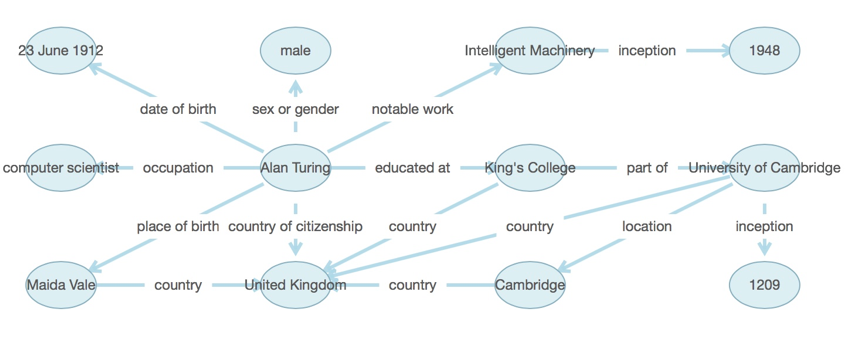
\includegraphics[width=0.80\textwidth]{kg.png}
    \caption{An Example Knowledge Graph}
    \label{fig:kg}
\end{figure}


The Questioner and The Answerer will talk in turns. They have freedom to choose how to phrase their sentences and keep the conversation natural, although, what they are talking about is constrained. Each turn, there will be a unique highlighted (red) relation in the graph together with a highlighted (green) node in this edge. The participants should only talk about the unique highlighted edge and node in each turn.

The Questioner is the initiator of the conversation. In order to start a conversation, Questioner should ask a question based on the relation (edge) in red. The node marked in green should be the answer of the question. The Questioner will send the natural language question together with the same graph with the same marking to the Answerer. After the Answerer received the question, he/she have to answer the question according to the marked graph and the conversation history so far. Then the Answerer will send the response to the Questioner and the marking on the graph will be updated according to a predefined script. Now the two participants have to start next turn. One import fact is the conversation history so far is always visible to both participants. Consequently, their utterance will always depend on the context of the on-going conversation.

\begin{figure}[h]
    \centering
    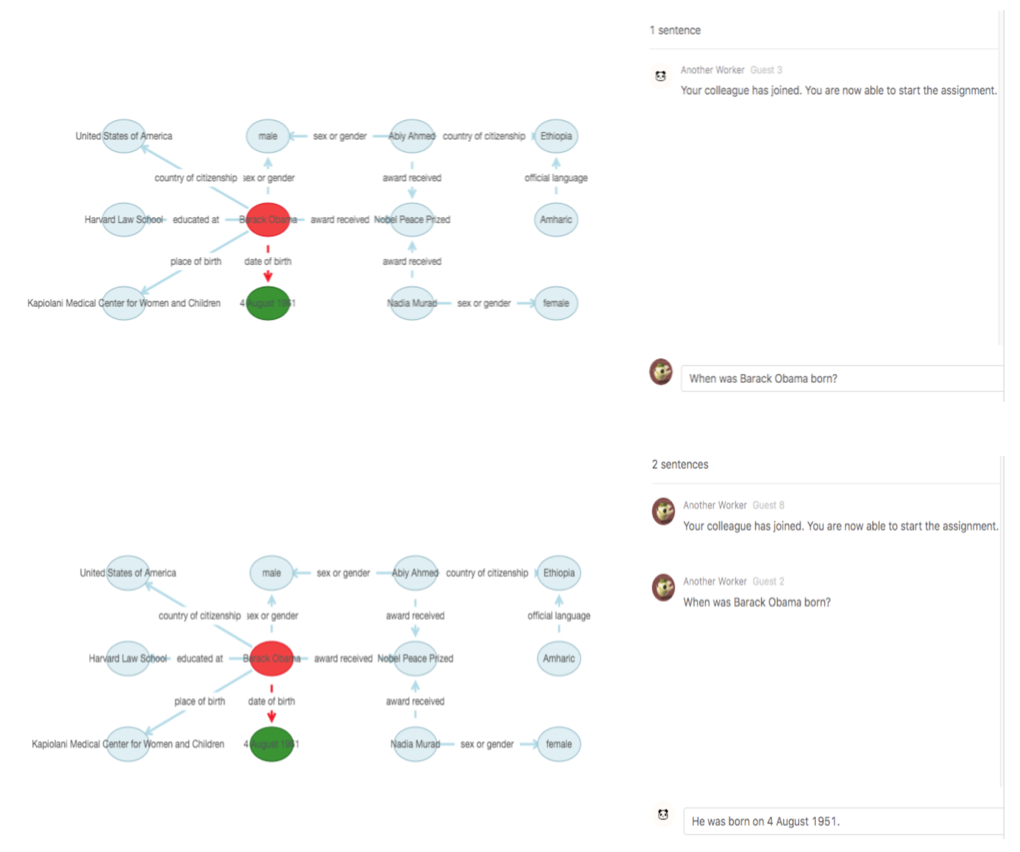
\includegraphics[width=0.8\textwidth]{qa1.png}
    \caption{Question Answering Interface for Questioner(above) and Answerer(below).}
    \label{fig:kgjson}
\end{figure}

The conversation will be automatically terminated after 6 turns. In addition, between different conversations, the underlying knowledge graph may be different, but remain the same within each conversation. During the experiment, participants are unable to see each other. There is no non-verbal commutation between the two participants and they are paid for this task.

\subsection{Corpus Description}

Our corpus consists of 240 coherent extended conversations collected via crowd-sourcing. Each conversation contains 6 turns and each turn composed of a natural language question and a natural language answer to that question. All utterances in a conversation are correlated on its prior context and the grounded knowledge graph and linked to the marking on knowledge graph of that turn. Figure\ref{fig:exampledata} is an example datapoint in our corpus.

\begin{figure}[h]
    \centering
    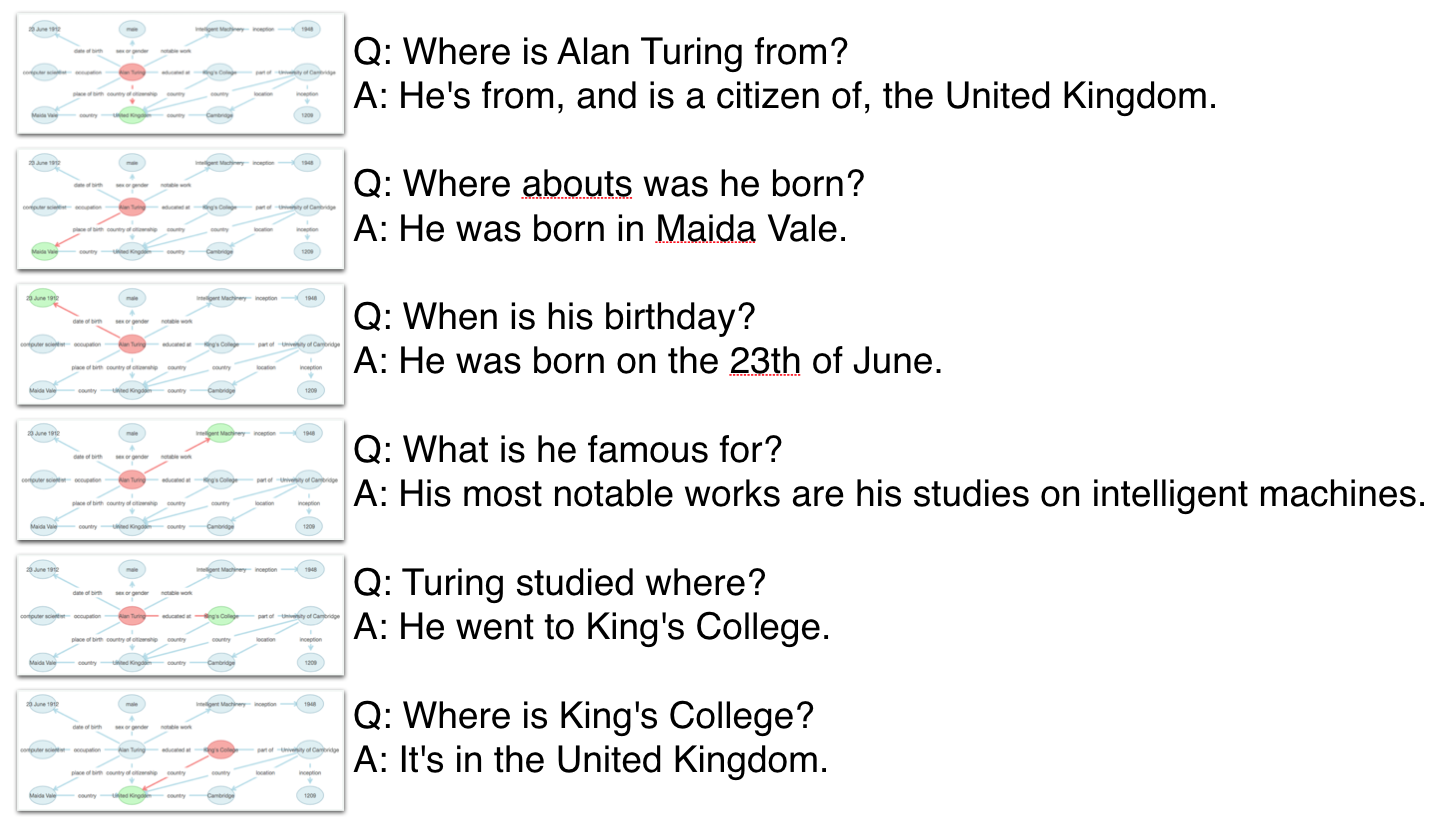
\includegraphics[width=0.8\textwidth]{eaxmppledata.png}
    \caption{An Example Collected Conversation and its Grounded Knowledge Graph.}
    \label{fig:exampledata}
\end{figure}

All the knowledge graphs are sampled from WikiData\cite{vrandevcic2014wikidata} and each graph has 12 nodes. The sequence of marking (highlighted relations and nodes) in each conversation is predefined by human annotators. Some demographic information of the participants, such as age, gender and nationalities, are collection under their permission. In addition, all the data entries are annotated with labels in Table\ref{tab:terms} and Table\ref{tab:tags} which will be discussed later in this section.




\subsection{Important Aspects of the Corpus}
\subsubsection*{Knowledge Graph as External Knowledge}

Instead of letting the participants to ask questions solely based on their prior common knowledge, external information as grounded knowledge is provided. Different people have different interpretation about the world, conversations based on participants' common knowledge often rely on implicit context about the participants. This brings additional challenge to produce dialogue state representations.

As I mentioned in Chapter 2, using images or text paragraph is not idea for modeling open domain coherent dialogues in a question answering setting\cite{strub2017end,shekhar2017foil,reddy2019coqa,zhou2018dataset,de2017guesswhat,das2017visual,das2017learning,reddy2019coqa}. In our framework, we use knowledge graph as our external knowledge base. There are many advantages for using knowledge graphs as the external knowledge:

\begin{figure}[h]
    \centering
    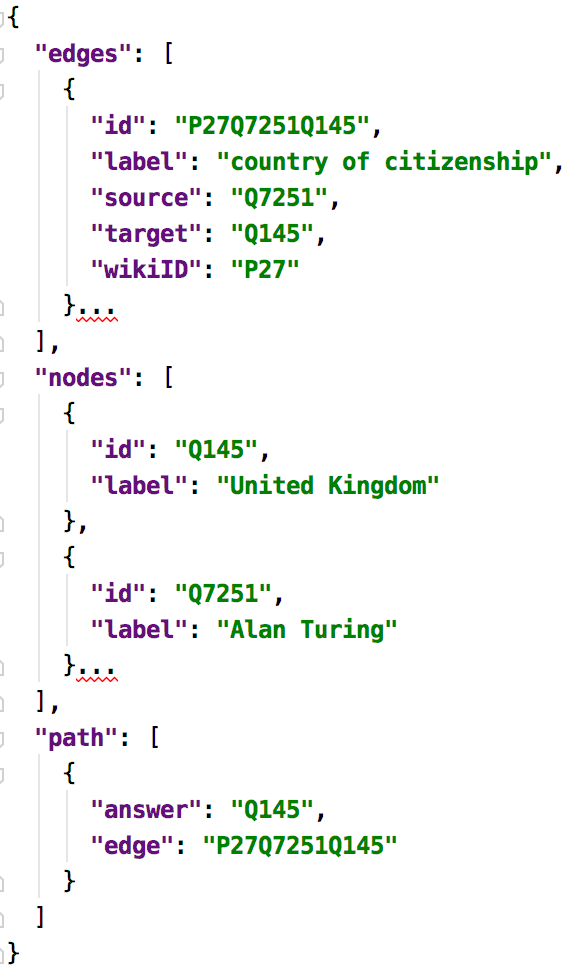
\includegraphics[width=0.4\textwidth]{gkjson.png}
    \caption{An Example Knowledge Graph in JSON Format}
    \label{fig:kgjson}
\end{figure}

\begin{enumerate}
   \item \textbf{Knowledge graph have two modalities.} 
   As illustrated in Figure\ref{fig:kgjson} and Figure\ref{fig:kg}, knowledge graph can be stored as structural data in the computer memory or visualized as an image graph. These two representations convey exactly the same information with different modalities. This provides both machine-readability and human-readability. By doing this, human participants don't outperform during the task and machines could learn effectively through the strong supervision signals it provided.
   
   \item \textbf{Knowledge graphs are unambiguous.} Different people have different way to interpret a sentence and label a text span. This makes the evaluation of the text-based question-answering task very challenging. As I mentioned above, human usually under-perform under such tasks. Unlike plain text, knowledge graph is unambiguous. Accurate evaluation is possible under this framework.
   
   \item  \textbf{Knowledge graphs are structural.} Knowledge graphs are structural in the sense that the relations between entities are easily interpretable. This makes it extremely easy to control the topic and topic switch of the conversations.
   
    \item \textbf{Knowledge graphs are open domain.} There are many existing knowledge graph datasets\cite{vrandevcic2014wikidata,bollacker2008freebase}. These knowledge graphs covers a wide range of topics which could be considered as open-domain.
    
    \item \textbf{Knowledge graphs are well-studied.} There are many prior works related to knowledge graphs, such as embedding\cite{lin2015learning}. In addition, a knowledge graph is a directed graph, there are many algorithms (e.g. depth first search) we could use for many purposes.
    

\end{enumerate}


As outlined above, knowledge graphs  is a good resource of external knowledge in our task. There are two popularly knowledge graphs which are widely used in literature, we decide to use WikiData\cite{vrandevcic2014wikidata} instead of Freebase\cite{bollacker2008freebase}. WikiData has an operating API. Researchers could directly query the API instead of dealing with raw data which can be hundreds of Gigabit.

\subsubsection*{Natural Conversation Grounded on Knowledge Graph}

For each conversation, there will be 6 relations and answer nodes highlighted in sequence. The sequence of the highlighted relations together with the highlighted node, which we call a path, is predefined in order to control the topic switches for each conversation. Different patterns of topic switches (paths) will have influence on the appearances of various linguistic patterns. In Table\ref{tab:terms}, I would like to introduce some terminologies before we investigate the relations between those two patterns. 


\begin{table}[]
\begin{tabular}{|l|l|}
\hline
Terms         & Definition                                                                                                                                                                                                                       \\ \hline
Gaps          & \begin{tabular}[c]{@{}l@{}}If there is no overlap between the entities in relations between the previous \\ turn and the current turn, then we label the current turn with ‘Gap’ label.\end{tabular}                             \\ \hline
Continuous    & A conversation with no gap is called continuous.                                                                                                                                                                                 \\ \hline
Discontinuous & A conversation with one or more gaps is called continuous.                                                                                                                                                                       \\ \hline
Links         & \begin{tabular}[c]{@{}l@{}}When two turns are talking about the same entity, we call the following \\ turn is linked to the previous turn if there is a strong correlation between \\ their grounded relationships.\end{tabular} \\ \hline
\end{tabular}
\caption{Definition for Graph Annotation}
\label{tab:terms}
\end{table}


We sampled 10 sub graphs from Wikidata in 10 distinct topics. For each subgraph, we generate 4 paths for each graph with different number of gaps and links in the path. By doing this, we would like to investigate under what situation, human tend to produce various linguistic patterns, particularly elided construction, in an extended coherent dialogue.


\subsubsection*{Annotations for Linguistics Patterns}

Each utterance in the corpus is tagged with various linguistics patterns by human annotators. There are eight such tags in our corpus. Four of them are considered to be class label. Consequently, tagging those tags is a classification task which the annotator see the whole utterance and annotate the tags to the whole sentence. The rest four tags are sequence labels, which these tags are labeled to a text span of the original utterance. Table\ref{tab:tags} summarizes the details about our tag set. All annotators are tagging the corpus according to the annotation schema in Appendix.  

% Please add the following required packages to your document preamble:
% \usepackage{multirow}
% \usepackage{graphicx}
\begin{table}[]
\centering
\resizebox{\textwidth}{!}{%
\begin{tabular}{|l|l|l|}
\hline
Type                            & Tag                                                                            & Definition                                                                                                                                                                                                                                                                                                                                                                                                                                                                                                       \\ \hline
\multirow{4}{*}{Classification} & Sluicing                                                                       & \begin{tabular}[c]{@{}l@{}}Sluicing is a type of ellipsis that occurs in both\\ direct and indirect interrogative clauses. The ellipsis\\ is introduced by a wh-expression, whereby in most\\ cases, everything except the wh-expression is elided\\ from the clause.\end{tabular}                                                                                                                                                                                                                               \\ \cline{2-3} 
                                & Anaphor                                                                        & \begin{tabular}[c]{@{}l@{}}Anaphora is the use of an expression whose\\ interpretation depends upon another expression in \\ context (its antecedent or postcedent). In our schema,\\ anaphora is the use of an expression that depends\\ specifically upon an antecedent expression.\end{tabular}                                                                                                                                                                                                               \\ \cline{2-3} 
                                & Short Answer                                                                   & \begin{tabular}[c]{@{}l@{}}Short answer (= answer fragments) is a type of\\ ellipsis that occurs in answers to questions. In\\ our schema, we define all answer utterances which\\ is not a fully grammatical sentence to be short answer.\end{tabular}                                                                                                                                                                                                                                                          \\ \cline{2-3} 
                                & Error                                                                          & \begin{tabular}[c]{@{}l@{}}Error tag should only be annotated when there is a\\ disagreement between the grounded knowledge graph\\ and the utterances.\end{tabular}                                                                                                                                                                                                                                                                                                                                             \\ \hline
\multirow{4}{*}{Labelling}      & \begin{tabular}[c]{@{}l@{}}Additional information\\ outside graph\end{tabular} & \begin{tabular}[c]{@{}l@{}}If parts of an utterance introduce additional information\\ into the conversation which is not mentioned in the\\ grounded knowledge graph, we call this part additional\\ information outside the knowledge graph.\end{tabular}                                                                                                                                                                                                                                                      \\ \cline{2-3} 
                                & \begin{tabular}[c]{@{}l@{}}Additional information\\ within graph\end{tabular}  & \begin{tabular}[c]{@{}l@{}}If parts of an utterance introduce additional information\\ into the conversation which is mentioned in the graph\\ and such information is not highlighted, we call them\\ additional information within the knowledge graph.\end{tabular}                                                                                                                                                                                                                                           \\ \cline{2-3} 
                                & Conversation Control                                                           & \begin{tabular}[c]{@{}l@{}}Conversation Control label should be tagged to any\\ pieces of utterance which functionally act as a\\ connector to make the whole conversation more\\ natural and coherent.\end{tabular}                                                                                                                                                                                                                                                                                             \\ \cline{2-3} 
                                & Totally Irrelevant                                                             & \begin{tabular}[c]{@{}l@{}}Totally irrelevant tag should be used when pieces of\\ utterance is totally irrelevant to the question answering\\ conversation. By deleting such pieces of information,\\ we will not influence the coherence of the conversation\\ or the meaning of the utterance. In addition, this tag should\\ only be considered if the part of utterance is not labelled as\\ other labels. In other words, labels, such as Conversation\\ Control, will have higher precedence.\end{tabular} \\ \hline
\end{tabular}%
}
\caption{Definition of Tag Set.}
\label{tab:tags}
\end{table}


\newpage
\section{Implementation}

This section introduces the tool-kits have been developed and used during this project. In addition, we brief discuss the technical difficulties and their solutions during the project.

\subsection{Sampling from Knowledge Graph}

In order sample sub-graphs from Wikidata, a Java toolkit named KnowledgeGraphClient is developed.

\begin{figure}[h]
    \centering
    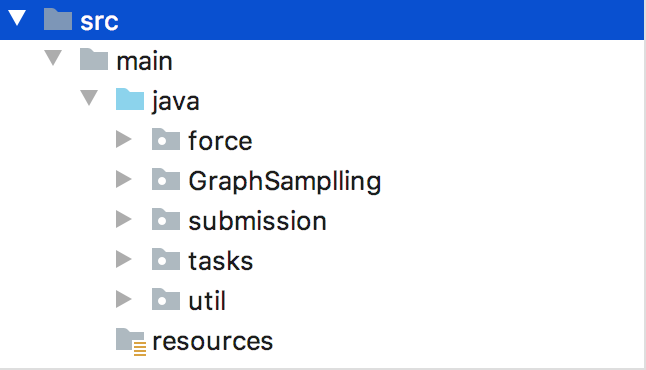
\includegraphics[width=0.4\textwidth]{client.png}
    \caption{Structure of KnowledgeGraphClient.}
    \label{fig:client}
\end{figure}

In order to interact with Wikidata, a Java package name Wikidata Toolkit\cite{wikitoolkit} is used. This package provide APIs to query Wikidata for entities (nodes in Figure\ref{fig:kg}) and relations relation to it.



A sub-graph is sampled via a depth-first search algorithm. We pre-defined a set of "interesting relations" which we only explore a connected node if the relation connecting that node and current node is in the set. We clearly don't want to include relations which are rarely mentioned in our daily life. For example, we would rarely talk about relations like: Obama is an instance of human and human is a subclass of animal. We start the search at a predefined node, for example, Obama(Q76). Q76 is the unique Wikidata ID for Obama. We potentially could traversal all nodes which are connected to Obama, however, I set the maximum depth of the search to be 4. In other words, we only explore nodes 4 connection away from the starting node. After the search, we would have a set of edges and nodes which will form a directed graph. In order to visualise the graph, I tried to apply force-directed algorithm to make reduce the overlap among these nodes.

\begin{figure}[h]
    \centering
    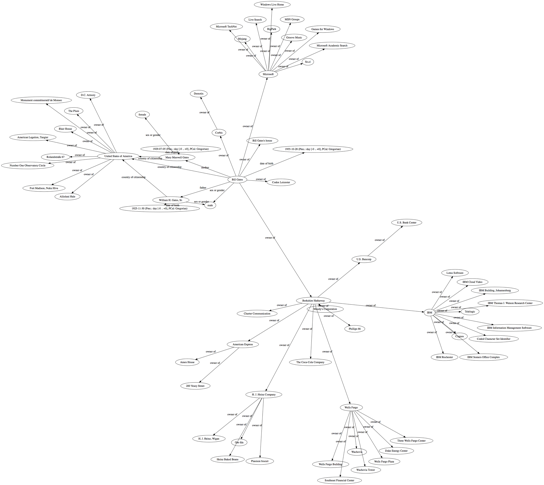
\includegraphics[width=0.4\textwidth]{directed.png}
    \caption{An Example Force-Directed Graph.}
    \label{fig:obama}
\end{figure}

However, such a graph is not very human interpretable and visible. I decided to follow a semi-automatic approach which I manually select nodes and edges from the above graph and directly give the coordinate for each node. In addition, the paths are also manually generated. By this approach, we generated 40 graphs in 10 distinct topics.

\subsection{Generating Questions from Knowledge Graph}

Instead of collecting dialogues from human participants, Indurthi et al.\cite{indurthi2017generating} has tried to automatically generate question answer pairs from a given knowledge graph. From each such set, they use a subset of keywords to generate a natural language question that has a unique answer. They treat this subset of keywords as a sequence and use an encoder-decoder model to generate natural questions from it.


\begin{table}[]
\centering
\begin{tabular}{|l|l|}
\hline
Predicate        & CEO           \\
Subject          & Sundar Pichai \\
Object           & Google        \\
Parent Predicate & designation   \\
Domain           & person        \\
Range            & organization  \\ \hline
\end{tabular}
\caption{An example set of keywords constructed from the triple(Sundar Pichai, CEO, Google)\cite{indurthi2017generating}}
\label{tab:keyword}
\end{table}

We re-implemented their experiment in a similar setting and the experiment results are shown in Table\ref{tab:genresult}. The larger model is a bi-directional RNN containing one hidden layer of 1000 units. We also build a small model, use a bi-directional RNN containing one hidden layer of 500 units due to the limitation of computation power. However, their method faces domain-adaption problem which could not produce grammatical sentences with out-domain data. Consequently, this dataset requires human intelligence and crowdsourcing is reqiured. 

\begin{table}[]
\centering
\begin{tabular}{|l|l|}
\hline
Models                 & BLEU Score \\ \hline
BiRNN-Large-Reported   & 50.14      \\ \hline
BiRNN-Small-Experiment & 38.45      \\ \hline
BiRNN-Large-Experiment & 49.72      \\ \hline
\end{tabular}
\caption{Experiment Result for Generating Conversation\cite{indurthi2017generating}}
\label{tab:genresult}
\end{table}

\newpage
\subsection{Web-interface for Data Collection}

In order to collect this corpus via crowd-sourcing, we built a web-interface together with a web server from scratch. A large proportion of our effort for this project have been spent into developing this software. There are two major challenges during the development: 1) This is a production system, which real users have to interact with this system. Consequently, the system has to be thoroughly tested. 2) Sometimes, human behaviour are unpredictable. It's very challenging to design and implement a robust system that could handle unexpected human behaviours.


\begin{figure}[h]
    \centering
    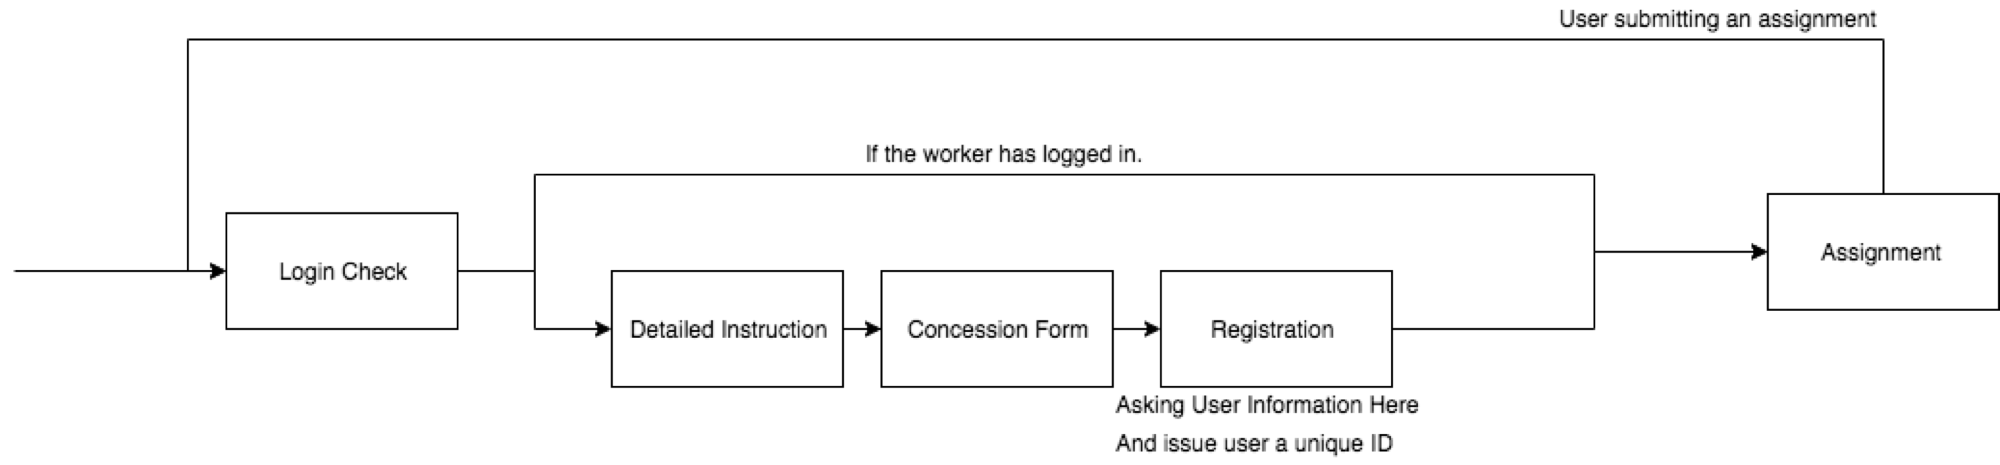
\includegraphics[width=0.9\textwidth]{process.png}
    \caption{The Workflow of the Web Interface.}
    \label{fig:web}
\end{figure}

As shown in Figure\ref{fig:web}, if a new user participates in our experiment, he/she will be shown a detailed instruction about the experiment. If the participant decides to take part in the experiment, he/she has to sign a consent form according to the data protection regulation. If the user agrees with the terms and conditions of the experiment, after registering an account, the user could see the web-page for our task. More detailed workflow and screen shots of this web interface are in appendix. In order to develop this web interface, we have used many packages.

\begin{table}[]
\centering
\begin{tabular}{|l|l|}
\hline
Package                  & Purpose                                                   \\ \hline
NodeJS\cite{nodejs}      & Writing Web-server.                                       \\ \hline
MongoDB\cite{monodb}     & Database for storing user information and collected data. \\ \hline
ReactJS\cite{react}      & Build user interfaces.                                    \\ \hline
AntD\cite{antd}           & Components for user interface.                  \\ \hline
G6\cite{g6}              & Rendering knowledge graphs in front end.                   \\ \hline
Socket.IO\cite{socketio} & Writing the socket server for online chatting.                \\ \hline
\end{tabular}
\caption{Packages Imported for Developing the Web-interface.}
\label{tab:packages}
\end{table}


\subsubsection{Tools for Annotating the Dataset}

In order to annotate the dataset, a toolkit named doccano\cite{doccano} is used. This is an easy to use web application which provides features for sequence to sequences tasks, classification tasks and sequence labelling tasks. Many other annotation tools have also been explored. However, most of them are professional and complicated to set up.

In addition, I develop a tool for post-processing and parsing our corpus which is frequently used during my data analysis.

\begin{figure}[h]
    \centering
    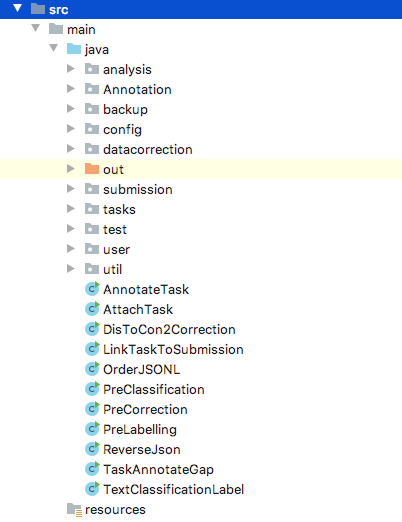
\includegraphics[width=0.4\textwidth]{parser.png}
    \caption{Toolkit for Post-processing and Parsing the Dataset.}
    \label{fig:parser}
\end{figure}



\newpage
\section{Data Collection Procedure}

In this section, we introduce how the corpus is collected. The whole data collection experiment runs for 2 months which is the most challenging and time-consuming part for this project. Totally 30 experiment sessions have been scheduled. The project is funded by Informatics Student Service and each participant will be paid a 5 pounds Amazon Voucher for their work. These are several constrains of the experiment which make organizing and running this experiment extremely hard.

\begin{enumerate}
   \item Each experiment session need two participants at the same time. 

   \item Only native speakers could participate in this experiment.
 
   \item Building a robust system that multiple users could interact with simultaneously is hard. 
       
\end{enumerate}


In this section, we discuss our data collection procedure in the following order: Advertising the Experiment and Scheduling the Experiment. Finally, I would like to give some advises for futures researchers who are aiming to collect a dialogue corpus in a lager scale.

\subsubsection*{Advertising the Experiment}

In order to recruit enough participants for this project, advertising this experiment is crucial. We have try several methods:

\begin{enumerate}
   \item Emailing the whole Informatics students.

   \item Pinning leaflet around the camps. 
 
   \item Posting advertisement on social medial (Facebook).
\end{enumerate}

Emailing students is the most effective approach which I recruit most of the participant from. An alternative approach is to deploy this experiment to crowdsourcing platform, such as Amazon Mechanic Turk\cite{mturk}. Hundreds of participants could be recruited overnight if the experiment is reasonably paid.


\subsubsection*{Scheduling the Experiment}

The most challenging part of the data collection and even the whole project is to schedule these experiment sessions. It is very difficult to pair up the participants and find a suitable time for both of them. We have tried to make a google form and ask participants to select their available time slots. We also he tried to send a group email to  all the interested participants and ask them if they are available for a fixed time session. Because people don't check their emails regularly, it takes time for our participants to reply. Consequently, all of the above approaches don't work well for our experiment.

Finally, we start following the this procedural and it works reasonably well.

\begin{enumerate}

    \item Participants have to be registered on a list if they are interested in his project.

   \item Build an online survey and ask participants roughly when are they available next week.

   \item Pair up participants who are available on the same data.
 
   \item Ask permission to share their emails with other participants.
   
    \item Send this pair of participants a group email and ask them to find a suitable time themselves.

    \item Confirm the attendance one day before the experiment session and send them a detailed instruction for that session.
    
\end{enumerate}

However, when the scale of the corpus goes larger (thousands of conversations), we strongly encourage researchers to hire full time in-house annotators, if the resource is available.

\section{Data Annotation Procedure}

The whole corpus is annotated by in-house annotators (my friends and I) according to an annotation schema (See Appendix). The majority of the annotation work is done by myself. A subset of the corpus (10\%) has been annotated twice by different annotators, in order to calculate the inter-annotator agreement. Cohen's Kappa is used for calculating the agreement between annotators.

\section{Compare to Previous Work}

Our corpus contains natural extended conversations grounded on an external wide-coverage structural knowledge graph. At present, there are no such datasets exist (see Table\ref{tab:compare}) and this is what our corpus mainly developed for.

% Please add the following required packages to your document preamble:
% \usepackage{graphicx}
\begin{table}[]
\centering
\resizebox{\textwidth}{!}{%
\begin{tabular}{|l|l|l|l|l|l|}
\hline
Dataset                           & Year & Multi-turn & Natural Conversation & Answer Type           & External Knowledge Type \\ \hline
CoQA\cite{reddy2019coqa}          & 2018 & \bluecheck & \bluecheck           & Text Span             & Text                    \\
CSQA\cite{saha2018complex}        & 2018 & \bluecheck & \xmark               & Text Answer           & Knowledge Graph         \\
SQuAD\cite{rajpurkar2016squad}    & 2016 & \xmark     & \xmark               & Text Span             & Wikipedia articles      \\
SQuAD 2.0\cite{rajpurkar2018know} & 2016 & \xmark     & \xmark               & Text Span             & Wikipedia articles      \\
QuAC\cite{choi2018quac}           & 2018 & \bluecheck & \xmark               & Text Span             & Wikipedia articles      \\
FiloIT\cite{shekhar2017foil}      & 2017 & \xmark     & \xmark               & Text Span             & Images                  \\
GuessWhat\cite{de2017guesswhat}   & 2017 & \bluecheck & \xmark               & Object Position       & Images                  \\ \hline
Our Dataset                       & 2020 & \bluecheck & \bluecheck           & Natural Text Response & Knowledge Graph         \\ \hline
\end{tabular}%
}
\caption{A Comparison between this Corpus with Existing Relevant Question Answering Corpora.}
\label{tab:compare}
\end{table}


\chapter{Analysis and Discussion}

In this chapter, we perform some quantitative and qualitative analysis based on our corpus. We made several hypothesis according to our observation and we test the significance of these hypothesis statistically using t-test.

\section{Summary of the Corpus}

In previous chapter, we introduce a novel conversational question answering corpus. Our corpus contains 240 natural conversations, each has 6 question-answering pairs, in 10 distinct topics. These conversations are divided into two categories: continuous and discontinuous. There are 140 continuous and 100 discontinues conversations. Discontinues conversations are additionally split into two subgroup, discontinuous1 (conversation with only one gap) and discontinuous2 (conversations with many gaps). There are 43 "dis1" conversations and 57 "dis2" conversations. Table\ref{tab:topiccount} shows a detailed count for conversations of each topics in each categories.

% Please add the following required packages to your document preamble:
% \usepackage{graphicx}
\begin{table}[]
\begin{tabular}{|l|l|l|l|l|}
\hline
Topics             & WikiData ID & Continuous & Discontinuous1 & Discontinuous2 \\ \hline
AlanTuring         & Q7251       & 13         & 6              & 5              \\ \hline
JKRowlin           & Q34660      & 14         & 6              & 6              \\ \hline
Knuth              & Q17457      & 19         & 0              & 6              \\ \hline
Obama              & Q76         & 9          & 5              & 6              \\ \hline
Berkshire Hathaway & Q217583     & 12         & 7              & 5              \\ \hline
Softbank           & Q201653     & 18         & 0              & 6              \\ \hline
Apple              & Q312        & 11         & 7              & 6              \\ \hline
CPU                & Q5300       & 19         & 0              & 7              \\ \hline
London             & Q84         & 12         & 5              & 6              \\ \hline
Tianjin            & Q1173       & 13         & 6              & 5              \\ \hline
\end{tabular}
\caption{Detailed Topics Count for the Corpus.}
\label{tab:topiccount}
\end{table}



Table\ref{tab:datacount} shows basic statistics for our corpus.

\begin{table}[]
\centering
\begin{tabular}{|l|l|}
\hline
Number of Dialogues & 240   \\ \hline
Number of Questions & 2.9K  \\ \hline
Number of Answers   & 2.9K  \\ \hline
Number of Words     & 1.8K  \\ \hline
Number of Tokens    & 15.2K \\ \hline
\end{tabular}
\caption{Counts of the Dataset.}
\label{tab:datacount}
\end{table}




\subsection*{Inter-Annotator Agreement of the Corpus}

Inter-annotator agreement is a measure of how well two (or more) annotators can make the same annotation decision for a certain category. Cohen's Kappa is used here for calculating the agreement score between two annotators. The higher agreement score for a tag, the more confident the tag is valid. High agreement scores are desirable properties for a corpus to demonstrate the good quality of its annotations. 

\begin{table}[]
\centering
\begin{tabular}{|l|l|l|}
\hline
Tag                                                                            & Cohen's Kappa & Agreement                \\ \hline
Anaphora                                                                       & 0.9476        & Almost perfect agreement \\ \hline
\begin{tabular}[c]{@{}l@{}}Short Answer\end{tabular}                         & 0.9370        & Almost perfect agreement \\ \hline
Error                                                                          & 0.0           & Slight agreement         \\ \hline
Sluicing                                                                       & 0.0           & Slight agreement         \\ \hline
\begin{tabular}[c]{@{}l@{}}Totally\\ Irrelevant\end{tabular}                   & 0.0           & Slight agreement         \\ \hline
\begin{tabular}[c]{@{}l@{}}Additional\\ information outside graph\end{tabular} & 0.3405        & Fair agreement           \\ \hline
\begin{tabular}[c]{@{}l@{}}Additional\\ information within graph\end{tabular}  & -0.0084(invalid)       & Poor agreement           \\ \hline
\begin{tabular}[c]{@{}l@{}}Conversation\\ Control\end{tabular}                 & 0.6060        & Moderate agreement       \\ \hline
\end{tabular}
\caption{Inter-annotator Agreement of the Corpus}
\label{tab:agree}
\end{table}

According to Table\ref{tab:agree}, Anaphora and Short Answer have a almost perfect agreement. Labels such as "Additional information outside graph" and "Conversation Control" have a lower Kappa score. This behaviour is expected and there are several reason:

\begin{enumerate}

    \item According to the annotation schema, the criteria for tags, such as Anaphora, is less ambiguous. Different interpretation of the semantics of the sentences usually doesn't influence on the judgment of that tag.
    
   \item There are obvious heuristics for tags, such as Anaphora and Sluicing. For example, the appearance of a pronoun may indicate the appearance of an anaphora and the appearance of a wh word indicates the possibility of a sluicing. 

   \item Tags, like Amphora, can usually be determined by the grammars instead of semantics of a sentence. 
 
   \item Annotating Amphora is a classification task, which is easier than a sequence labelling task.
   
   \item Annotators have to make inference about the conversation context in order to make a decision for tags like "Additional information within graph".
   
\end{enumerate}

In addition, we noticed that the Kappa score is 0.0 for many tags. Some tags are extremely sparse in the corpus and many rarely appear within the 10\% of the dataset.

\subsection*{Demographic of the Participants}

There are totally 17 native English speakers involved in our experiment. 7 of them are female and 10 of them are male. The majority of the participants (11) are from the United Kingom, 4 participants are from Singapore and 2 participants are from the United States. All participants are students from the University of Edinburgh and all of them are between 18 and 24.

\section{Statistical Analysis}

In this section, we perform some statistical analysis on the dataset. We additionally make some hypothesises according to our observations. The significance of each hypothesises is tested via t-test.

Table\ref{tab:ori} shows the count of each tags in the whole corpus. In this table, the filed of "Condition" is empty. This means all numbers in that table are subject to the whole corpus. If the filed of "Condition" is "Question", it means we only consider all the questions in this table. This filed acts like a filter for the dataset. In the table, it shows how many utterances satisfies the given "Condition". It also shows that how many utterances contain each tag and the proportion of the utterances with that tag in the utterances satisfies the "Condition". For example, Table\ref{tab:ori} shows that there are 2880 utterances in the dataste. 1197 of them contain Anaphora tag which consisit 41.56\% of thses utterances.

\begin{table}[]
\centering
\begin{tabular}{|l|l|l|}
\hline
Condition                            & \multicolumn{2}{l|}{}            \\ \hline
Total Number of Uutterance           & \multicolumn{2}{l|}{2880}        \\ \hline
Tags                                 & Count & Proportion per Utterance \\ \hline
Anaphora                             & 1197  & 0.4156                   \\ \hline
Short Answer                         & 902   & 0.3132                   \\ \hline
Error                                & 11    & 0.0038                   \\ \hline
Sluicing                             & 27    & 0.0094                   \\ \hline
Additional information outside graph & 50    & 0.0174                   \\ \hline
Additional information within graph  & 26    & 0.0090                   \\ \hline
Conversation Control                 & 181   & 0.0628                   \\ \hline
Totally Irrelevant                   & 26    & 0.0090                   \\ \hline
\end{tabular}
\caption{Statistics of Tags for the Corpus }
\label{tab:ori}
\end{table}




\begin{minipage}{\textwidth}
        \begin{minipage}[t]{0.45\textwidth}
            \centering
            \makeatletter\def\@captype{table}\makeatother
\resizebox{\textwidth}{!}{%
\begin{tabular}{|l|l|l|}
\hline
Condition                            & \multicolumn{2}{l|}{Continuous}  \\ \hline
Total Number of Uutterance           & \multicolumn{2}{l|}{1680}        \\ \hline
Tags                                 & Count & Proportion per Utterance \\ \hline
Anaphora                             & 737   & 0.4387                   \\ \hline
Short Answer                         & 529   & 0.3149                   \\ \hline
Error                                & 6     & 0.0036                   \\ \hline
Sluicing                             & 25    & 0.0149                   \\ \hline
Additional information outside graph & 41    & 0.0185                   \\ \hline
Additional information within graph  & 9     & 0.0054                   \\ \hline
Conversation Control                 & 104   & 0.0619                   \\ \hline
Totally Irrelevant                   & 13    & 0.0077                   \\ \hline
\end{tabular}%
}
\caption{Statistics of Tags for Continuous  Conversations.}
\label{tab:con}
        \end{minipage}
        \begin{minipage}[t]{0.45\textwidth}
        \centering
        \makeatletter\def\@captype{table}\makeatother
\resizebox{\textwidth}{!}{%
\begin{tabular}{|l|l|l|}
\hline
Condition                            & \multicolumn{2}{l|}{Discontinuous} \\ \hline
Total Number of Uutterance           & \multicolumn{2}{l|}{1200}          \\ \hline
Tags                                 & Count  & Proportion per Utterance  \\ \hline
Anaphora                             & 460    & 0.3833                    \\ \hline
Short Answer                         & 373    & 0.3108                    \\ \hline
Error                                & 5      & 0.0042                    \\ \hline
Sluicing                             & 2      & 0.0017                    \\ \hline
Additional information outside graph & 19     & 0.0158                    \\ \hline
Additional information within graph  & 17     & 0.0142                    \\ \hline
Conversation Control                 & 77     & 0.0642                    \\ \hline
Totally Irrelevant                   & 13     & 0.0108                    \\ \hline
\end{tabular}%
}
\caption{Statistics of Tags for DIscontinuous  Conversations.}
\label{tab:dis}
        \end{minipage}
    \end{minipage}





\begin{minipage}{\textwidth}
        \begin{minipage}[t]{0.45\textwidth}
            \centering
            \makeatletter\def\@captype{table}\makeatother
\resizebox{\textwidth}{!}{%
\begin{tabular}{|l|l|l|}
\hline
Condition                            & \multicolumn{2}{l|}{Discontinuous1} \\ \hline
Total Number of Uutterance           & \multicolumn{2}{l|}{516}            \\ \hline
Tags                                 & Count   & Proportion per Utterance  \\ \hline
Anaphora                             & 242     & 0.4690                    \\ \hline
Short Answer                         & 153     & 0.2965                    \\ \hline
Error                                & 0       & 0.0000                    \\ \hline
Sluicing                             & 1       & 0.0019                    \\ \hline
Additional information outside graph & 14      & 0.0271                    \\ \hline
Additional information within graph  & 9       & 0.0174                    \\ \hline
Conversation Control                 & 51      & 0.0988                    \\ \hline
Totally Irrelevant                   & 5       & 0.0097                    \\ \hline
\end{tabular}%
}
\caption{Statistics of Tags for Discontinuous 1  Conversations.}
\label{tab:dis1}

        \end{minipage}
        \begin{minipage}[t]{0.45\textwidth}
        \centering
        \makeatletter\def\@captype{table}\makeatother
\resizebox{\textwidth}{!}{%
\begin{tabular}{|l|l|l|}
\hline
Condition                            & \multicolumn{2}{l|}{Discontinuous2} \\ \hline
Total Number of Uutterance           & \multicolumn{2}{l|}{684}            \\ \hline
Tags                                 & Count   & Proportion per Utterance  \\ \hline
Anaphora                             & 218     & 0.0387                    \\ \hline
Short Answer                         & 220     & 0.3216                    \\ \hline
Error                                & 5       & 0.0073                    \\ \hline
Sluicing                             & 1       & 0.0015                    \\ \hline
Additional information outside graph & 5       & 0.0073                    \\ \hline
Additional information within graph  & 8       & 0.0117                    \\ \hline
Conversation Control                 & 26      & 0.0380                    \\ \hline
Totally Irrelevant                   & 8       & 0.0017                    \\ \hline
\end{tabular}%
}
\caption{Statistics of Tags for Discontinuous 2  Conversations.}
\label{tab:dis2}

        \end{minipage}
    \end{minipage}



According to our experiment design in Chapter 3, gaps represent non-connected topic shifts. The more non-connected topic shifts a conversation have, the less coherent it is. In our corpus, discontinuous1 (dis1) conversation has only one gap per conversation. Dis1 conversations represent conversations which the underlining logic is less coherent but still logistical. In contrast, discontinuous2 (dis2) conversations have many gaps, which the underlying logic is totally random.  

According to Table\ref{tab:con} - \ref{tab:dis2}, we make the following observation and hypothesis.

\begin{observation}
The continuity and coherence have influences on these linguistic patterns. However, the influence is not influence.
\end{observation} 

\begin{hypo}
In our corpus, answers are always related to their questions. Gaps will have little influence on answers. This smooths out the number.
\end{hypo}



In order to proof the check hypothesis, we additionally check the difference about the count of tags between questions and answers for both continuous and discontinuous conversations. Table\ref{tab:conque} - \ref{tab:disans} demonstrate the results. These results show obvious differences between the appearance of labels in questions and no obvious differences in answers. This obey the above hypothesis. Consequently, for the following statistics, we will focus on questions instead of answers.



\begin{minipage}{\textwidth}
        \begin{minipage}[t]{0.45\textwidth}
            \centering
            \makeatletter\def\@captype{table}\makeatother
\resizebox{\textwidth}{!}{%
\begin{tabular}{|l|l|l|}
\hline
Condition                            & \multicolumn{2}{l|}{Continuous  Question} \\ \hline
Total Number of Uutterance           & \multicolumn{2}{l|}{840}                  \\ \hline
Tags                                 & Count      & Proportion per Utterance     \\ \hline
Anaphora                             & 465        & 0.5536                       \\ \hline
Short Answer                         & 0          & 0.0000                       \\ \hline
Error                                & 3          & 0.0036                       \\ \hline
Sluicing                             & 25         & 0.0298                       \\ \hline
Additional information outside graph & 14         & 0.0167                       \\ \hline
Additional information within graph  & 2          & 0.0024                       \\ \hline
Conversation Control                 & 70         & 0.0833                       \\ \hline
Totally Irrelevant                   & 6          & 0.0071                       \\ \hline
\end{tabular}%
}
\caption{Statistics of Tags for Continuous  Questions.}
\label{tab:conque}

        \end{minipage}
        \begin{minipage}[t]{0.45\textwidth}
        \centering
        \makeatletter\def\@captype{table}\makeatother
\resizebox{\textwidth}{!}{%
\begin{tabular}{|l|l|l|}
\hline
Condition                            & \multicolumn{2}{l|}{Discontinuous  Question} \\ \hline
Total Number of Uutterance           & \multicolumn{2}{l|}{600}                    \\ \hline
Tags                                 & Count       & Proportion per Utterance      \\ \hline
Anaphora                             & 251         & 0.4183                        \\ \hline
Short Answer                         & 0           & 0.0000                        \\ \hline
Error                                & 4           & 0.0067                        \\ \hline
Sluicing                             & 2           & 0.0033                        \\ \hline
Additional information outside graph & 9           & 0.0150                        \\ \hline
Additional information within graph  & 7           & 0.0117                        \\ \hline
Conversation Control                 & 53          & 0.0833                        \\ \hline
Totally Irrelevant                   & 4           & 0.0067                        \\ \hline
\end{tabular}%
}
\caption{Statistics of Tags for Discontinuous Questions.}
\label{tab:disque}

        \end{minipage}
    \end{minipage}




\newpage
\begin{minipage}{\textwidth}
        \begin{minipage}[t]{0.45\textwidth}
            \centering
            \makeatletter\def\@captype{table}\makeatother
\resizebox{\textwidth}{!}{%
\begin{tabular}{|l|l|l|}
\hline
Condition                            & \multicolumn{2}{l|}{Continuous Answer} \\ \hline
Total Number of Uutterance           & \multicolumn{2}{l|}{840}               \\ \hline
Tags                                 & Count    & Proportion per Utterance    \\ \hline
Anaphora                             & 272      & 0.3238                      \\ \hline
Short Answer                         & 529      & 0.6298                      \\ \hline
Error                                & 3        & 0.0036                      \\ \hline
Sluicing                             & 0        & 0.0000                      \\ \hline
Additional information outside graph & 17       & 0.0202                      \\ \hline
Additional information within graph  & 7        & 0.0083                      \\ \hline
Conversation Control                 & 34       & 0.0405                      \\ \hline
Totally Irrelevant                   & 7        & 0.0150                      \\ \hline
\end{tabular}%
}
\caption{Statistics of Tags for Continuous Answers.}
\label{tab:conans}

        \end{minipage}
        \begin{minipage}[t]{0.45\textwidth}
        \centering
        \makeatletter\def\@captype{table}\makeatother
\resizebox{\textwidth}{!}{%
\begin{tabular}{|l|l|l|}
\hline
Condition                            & \multicolumn{2}{l|}{Discontinuous Answer} \\ \hline
Total Number of Uutterance           & \multicolumn{2}{l|}{600}                  \\ \hline
Tags                                 & Count      & Proportion per Utterance     \\ \hline
Anaphora                             & 209        & 0.3483                       \\ \hline
Short Answer                         & 373        & 0.6217                       \\ \hline
Error                                & 1          & 0.0017                       \\ \hline
Sluicing                             & 0          & 0.0000                       \\ \hline
Additional information outside graph & 10         & 0.0167                       \\ \hline
Additional information within graph  & 10         & 0.0167                       \\ \hline
Conversation Control                 & 24         & 0.0400                       \\ \hline
Totally Irrelevant                   & 9          & 0.0067                       \\ \hline
\end{tabular}%
}
\caption{Statistics of Tags for Discontinuous Answers.}
\label{tab:disans}

        \end{minipage}
    \end{minipage}


According to Table\ref{tab:conque} and Table\ref{tab:disque}, we find that:

\begin{observation}
Coherence and continuity of a conversation has an obvious influence on Anaphora and Sluicing.
\end{observation}

\begin{observation}
To answers, short answer and anaphora are not very sensitive to the coherence of the conversation. It may also because that the answer is always related to the question. 
\end{observation}


Based on the above observation, we believe that the gaps in discontinuous majorly influence the appearance of Anaphor and Sluicing. Intuitively, gaps represent non-connected topic shifts, which usually introduce additional entities into the conversation context. The appearance of these additional entities makes the co-reference resolution more difficult because determining which entity the pronoun refers to in the context is more ambiguous. Human may decide use less pronouns in this case. We compare the appearance of anaphora and sluicing between utterances without gaps and utterances with gaps. The results are shown in Table\ref{tab:quenogap} and Table\ref{tab:quegap}.


\begin{minipage}{\textwidth}


        \begin{minipage}[t]{0.45\textwidth}
            \centering
            \makeatletter\def\@captype{table}\makeatother


\resizebox{\textwidth}{!}{%
\begin{tabular}{|l|l|l|}
\hline
Condition                            & \multicolumn{2}{l|}{Question without Gap} \\ \hline
Total Number of Uutterance           & \multicolumn{2}{l|}{993}                  \\ \hline
Tags                                 & Count      & Proportion per Utterance     \\ \hline
Anaphora                             & 675        & 0.6798                       \\ \hline
Short Answer                         & 0          & 0.0000                       \\ \hline
Error                                & 3          & 0.0030                       \\ \hline
Sluicing                             & 26         & 0.0262                       \\ \hline
Additional information outside graph & 16         & 0.0161                       \\ \hline
Additional information within graph  & 4          & 0.0040                       \\ \hline
Conversation Control                 & 99         & 0.0997                       \\ \hline
Totally Irrelevant                   & 8          & 0.0081                       \\ \hline
\end{tabular}%
}
\caption{Statistics of Tags for Questions without Gaps.}
\label{tab:quenogap}



        \end{minipage}
        \begin{minipage}[t]{0.45\textwidth}
        \centering
        \makeatletter\def\@captype{table}\makeatother



\resizebox{\textwidth}{!}{%
\begin{tabular}{|l|l|l|}
\hline
Condition                            & \multicolumn{2}{l|}{Question with Gap} \\ \hline
Total Number of Uutterance           & \multicolumn{2}{l|}{447}               \\ \hline
Tags                                 & Count    & Proportion per Utterance    \\ \hline
Anaphora                             & 41       & 0.0917                      \\ \hline
Short Answer                         & 0        & 0.0000                      \\ \hline
Error                                & 4        & 0.0089                      \\ \hline
Sluicing                             & 1        & 0.0022                      \\ \hline
Additional information outside graph & 7        & 0.0157                      \\ \hline
Additional information within graph  & 5        & 0.0112                      \\ \hline
Conversation Control                 & 24       & 0.0537                      \\ \hline
Totally Irrelevant                   & 2        & 0.0081                      \\ \hline
\end{tabular}%
}
\caption{Statistics of Tags for Questions with Gaps.}
\label{tab:quegap}


        \end{minipage}
    \end{minipage}


According to Table\ref{tab:quenogap} and Table\ref{tab:quegap}, we have following observation. Based on this observation, we make two hypotheses. 

\begin{observation}
Gaps have an obvious influence on Anaphor and Sluicing. It is much more anaphor and sluicing appear in questions without gaps.
\end{observation}

Based on this observation, we make two hypothesis.

\begin{hypo}
Gaps have influences on Anaphor. An utterance is more likely to contain anaphora without a gap. 
\end{hypo}

The T-test score for this hypothesis is 5.3805E-106. This score reject the null hypothesis which there is a very little probability, the above hypothesis happens by chance. We prove that the above statement is statistically significant. We also have similar statement for Sluicing.

\begin{hypo}
Gaps have influences on anaphor. An utterance is more likely to contain anaphora without a gap. 
\end{hypo}

The T-test score for this hypothesis is 4.1702E-8 which also demonstrates the significance of the above hypothesis.

We additionally interested in the effect of links to these tags. 



\begin{minipage}{\textwidth}


        \begin{minipage}[t]{0.45\textwidth}
            \centering
            \makeatletter\def\@captype{table}\makeatother


\resizebox{\textwidth}{!}{%
\begin{tabular}{|l|l|l|}
\hline
Condition                            & \multicolumn{2}{l|}{Linked Question without Gap} \\ \hline
Total Number of Uutterance           & \multicolumn{2}{l|}{98}                          \\ \hline
Tags                                 & Count         & Proportion per Utterance         \\ \hline
Anaphora                             & 63            & 0.6429                           \\ \hline
Short Answer                         & 0             & 0.0000                           \\ \hline
Error                                & 0             & 0.0000                           \\ \hline
Sluicing                             & 21            & 0.2143                           \\ \hline
Additional information outside graph & 2             & 0.0204                           \\ \hline
Additional information within graph  & 0             & 0.0000                           \\ \hline
Conversation Control                 & 13            & 0.1327                           \\ \hline
Totally Irrelevant                   & 0             & 0.0000                           \\ \hline
\end{tabular}%
}
\caption{Statistics of Tags for Linked Questions without Gaps.}
\label{tab:quegaplink}


        \end{minipage}
        \begin{minipage}[t]{0.45\textwidth}
        \centering
        \makeatletter\def\@captype{table}\makeatother


\resizebox{\textwidth}{!}{%
\begin{tabular}{|l|l|l|}
\hline
Condition                            & \multicolumn{2}{l|}{Unlinked Question without Gap} \\ \hline
Total Number of Uutterance           & \multicolumn{2}{l|}{895}                           \\ \hline
Tags                                 & Count          & Proportion per Utterance          \\ \hline
Anaphora                             & 612            & 0.6838                            \\ \hline
Short Answer                         & 0              & 0.0000                            \\ \hline
Error                                & 3              & 0.0034                            \\ \hline
Sluicing                             & 5              & 0.0056                            \\ \hline
Additional information outside graph & 14             & 0.0156                            \\ \hline
Additional information within graph  & 4              & 0.0045                            \\ \hline
Conversation Control                 & 86             & 0.0961                            \\ \hline
Totally Irrelevant                   & 8              & 0.0089                            \\ \hline
\end{tabular}%
}
\caption{Statistics of Tags for Unlinked Questions without Gaps.}
\label{tab:quegapnolink}

        \end{minipage}
    \end{minipage}


From Table\ref{tab:quegaplink} and Table\ref{tab:quegapnolink}, we observe that:

\begin{observation}
Links have an obvious influence on sluicing. Links don't have an obvious influence on anaphor.
\end{observation}

Based on this observation, we make two hypothesises:

\begin{hypo}
Links have an influence on the appearance of sluicing. A linked question is more likely to contain a sluicing construciton.
\end{hypo}

The T-test score for this hypothesis is 1.3983E-9. The none hypothesis is rejected which demonstrates the significance of the above hypothesis.

We would also prove that there is no obvious relation between links and anaphora.

\begin{hypo}
Links have an influence on the appearance of anaphora.
\end{hypo}

This hypothesis is rejected by achieving a t-test score of 0.4226. It means that there is 42.26\% probability the pattern we observed in the hypothesis happens by chance. In other words, there is no sufficient evidence to show there is a correlation between the appearance of links and the appearance of sluicing.

Not only for elided construction, the above statistics also demonstrates that people also try to introduce additional utterances to connect gaps between each turns. However, people sometimes give up when the conversations are totally incoherent.


\chapter{Modelling Coherent Dialogues Using Neural Networks}

In order to model the coherent dialogues in this corpus, we proposed a novel neural architecture. However, this model is not implemented due to the scale of this project. The corpus only contains 240 conversations. As I argued in Chapter 2, this may be insufficient to train such a complicated neural network. In this chapter, we introduce our proposed framework to train a neural dialogue models if the resources are available in the future.

\section{Hierarchical Attentional Encoder with Context Windows}

In order to encode coherent dialogue, we need to model long-distance dependencies not only between words in one utterance, but also between sentences within the discourse. For example, in order to model an elided construction, our model has to infer the omission from the longer prior context of the conversation, because such information may not appear in the current utterance. To model that, we propose a hierarchical attentional encoder which is inspired by Xing et al. \cite{xing2018hierarchical}. We extend their model with context windows which the size of the windows is a predefined hyper-parameter to control how many previous turns we are modelling. 


\begin{figure}[h]
    \centering
    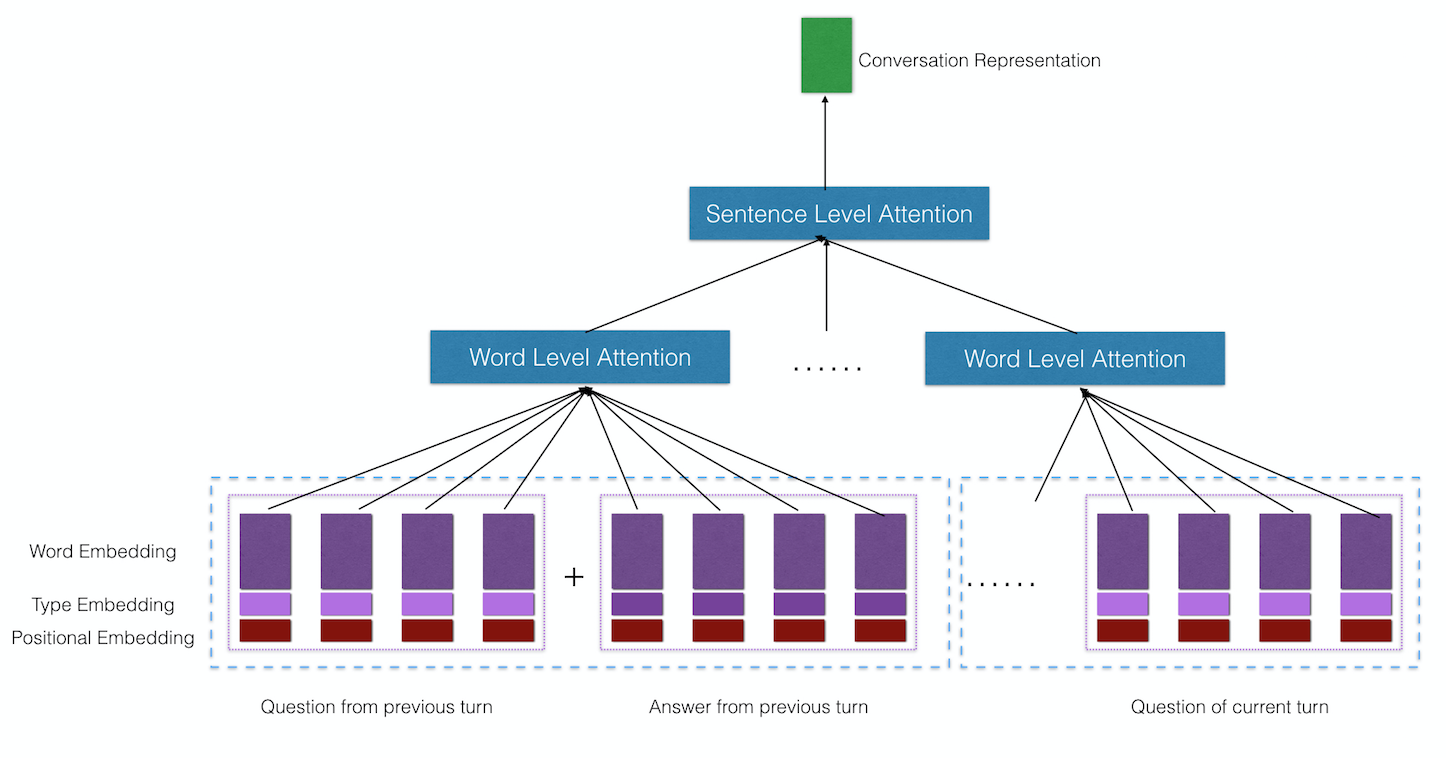
\includegraphics[width=0.75\textwidth]{attemodel.png}
    \caption{Hierarchical Attentional Encoder with Context Window.}
    \label{fig:mesh1}
\end{figure}

We would like to use BERT\cite{devlin2018bert} to provide a contextual embedding for each word. Additional turn embedding is used to denote the turn and type of a sentence. The concatenated embedding is fed into a self-attentional layer which models the dependencies within the context window. Additional sentence level attention will be used to model the dependencies between context windows. In addition, we will adapt a multi-modal deep neural network architecture to produce the dialogue state representation for downstream tasks.

\begin{figure}[h]
    \centering
    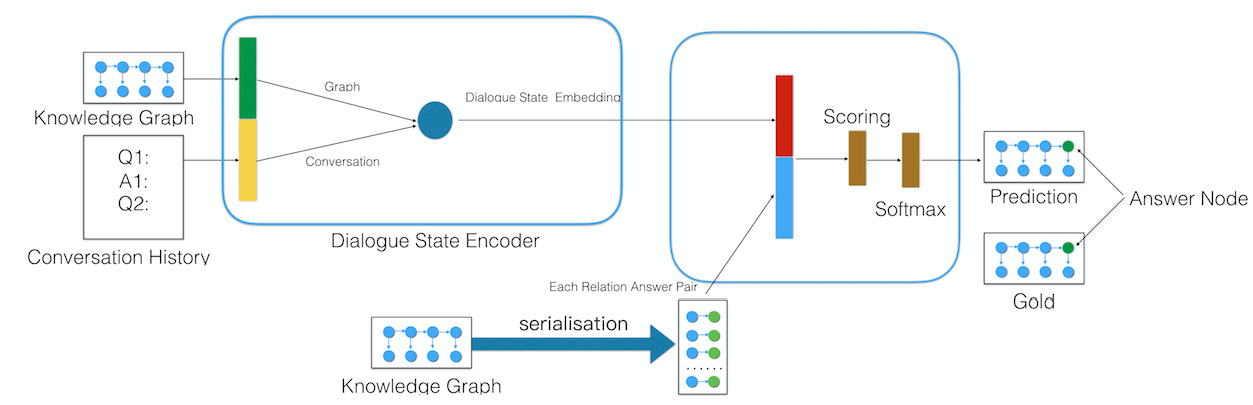
\includegraphics[width=0.85\textwidth]{qa1pro.png}
    \caption{The Multi-modal Question Answering Architecture.}
    \label{fig:mesh1}
\end{figure}


To predict the correct node to answer a given question, we could represent a prediction as a quadruple, such as, (Subject Node, Relation, Object Node, Position of the Answer). An example of the prediction could be (Barack Obama, born, 1967, object) which corresponds to the question ``When was Obama born?". We permute all the possible combinations within the graph. Then we use a feed-forward neural network together with a softmax layer to produce a multinomial distribution over all the possible answers. Then the prediction is compared with the gold answer and we could calculate the reward or loss to train our model.

\subsection{Generate Coherent Dialogues as a Markov Decision Process}
\noindent
As we argued in chapter 2, training a dialogue system with supervised learning is not explicitly optimized to produce a coherent response. We propose to cast the response generation task as a RL task. More specifically, we consider the questioner and the answerer as part of the RL agent environment. According to Williams and Young\cite{williams2007partially}, a goal-driven dialogue system could be modelled as a partially observable Markov decision process. Inspired by Strub et al. \cite{strub2017end}, We would like to describe our response generation task as following:

We define the state $S_t$ as the state of the dialogue at step t. An action $u_t$ corresponds to selecting a new word in the vocabulary V. The transition to the next state depends on the selected action:

\begin{itemize}
\item If we generate the end of sentence token . , the ongoing response is terminated and the next question is sampled from the questioner.
\item Otherwise the new word is appended to the ongoing answer.
\end{itemize}

A dialogue is started with an initial question and finished after a fixed number of turns. A reward is defined for every state action pair. 

\subsection{Extrinsic Evaluation of Dialogue Models}
\noindent

We will use precision and recall, which are well-established metrics for question answering tasks, as our extrinsic evaluation metrics. In our framework, high precision and recall demonstrate a good performance of modelling the linguistic patterns within a coherent dialogue.





\chapter{Conclusion}


\section{Summary}

In this project, we first briefly introduce the history and development of dialogue systems in terms of rule-based system, corpus-based systems and the architecture of the state of the art spoken dialogue systems. Then we discuss the important distinctions between different dialogue corpora: whether the corpus features constrained or unconstrained dialogues; whether a corpus is written, spoken; whether a corpus features human-human interactions or human-machine interactions. Afterwards, we review the publicly available corpora for training dialogue systems. We also investigate Intrinsic Evaluation, Extrinsic Evaluation and Human Evaluation methods for dialogue system evaluation and discuss the pros and cons of each approach.

The motivation for this project is to build a coherent open-domain dialogue systems with neural networks. To the best of our knowledge, there is no publicly available corpus suitable on training coherent open-domain dialogue models. To achieve this goal, we design and collect a novel corpus contains extended coherent dialogues of questions and responses that are information in a knowledge graph. These dialogues describe the relations within a knowledge graph with clear links between the phrases in the questions to nodes in a knowledge graph. The purpose for this corpus is to perform statistical analysis about various linguistic patterns within coherent dialogues, thereby, create a framework for neural models to learn how to parse these patterns and produce more coherent responses. This corpus has been collected via crowd-sourcing. The dialogue collection experiment was running for 3 months which 30 sessions have been organized. In order to prepare this experiment, several toolkits have been developed.

The main focus for this project is to investigate when the appearance of an elided construction is natural and convey the intended content. A detailed statistical analysis have been conducted on this corpus. We find:

\begin{enumerate}
   \item Gaps have influences on anaphor and sluicing. An utterance is more likely to contain these patterns without a gap.

   \item Links have an obvious influence on sluicing however links don’t have an obvious influence on anaphor.
 
\end{enumerate}

We prove the statistical significance of those hypothesis on our corpus.

\section{Future Work}

Due to the scale of this project and the limitation of the available resources, only 240 conversations have been collected in the corpus. In order to train decent dialogue models using deep neural networks, a larger corpus should be collected. For collecting a larger corpus, both the topics of the knowledge graphs and tags in our tag set should be further diversified.

During this project, we have implemented a web interface for this task-specific dialogue collection experiment. This interface is for single purpose. A general purpose toolkit for crowd sourcing goal-orientated dialogue corpora should be developed. This toolkit should facilitate researchers to design, create and deploy such tasks into crowd sourcing platforms, such as Amazon Mechanic Turk\cite{mturk}. There are existing similar toolkits\cite{lee2018dialcrowd,miller2017parlai}, it's not easy enough to create a similar experiment by only using these tools.

In chapter 5, we proposed a hierarchical attentional neural architecture with context windows. Training such a neural model under our framework may improvement the performance of current spoken dialogue systems. Although the current statistical SDSs do explicitly capture the dialogue history via belief tracking, they may not utilize rich linguistic information inside a coherent dialogue\cite{gasic}. Future study could integrate a conversation model into the semantic decoder and encoder to enable the current SDSs to understand and produce more coherent dialogues. In addition, current SDSs require pre-defined ontology in order to keep track of the belief state. Researcher could investigate whether we could connect a SDS to a wide coverage knowledge graph and build a dialogue system which can support a natural conversation about any topic within the knowledge graph. Cheng et al.\cite{cheng2019learning} has developed a transition-base neural semantic parser with a generic tree-generation algorithm. By integrating a conversation model with an existing neural semantic parser, we may enable it to perform semantic parsing over an extended coherent dialogue.



% use the following and \cite{} as above if you use BibTeX
% otherwise generate bibtem entries
\bibliographystyle{plain}
\bibliography{mybibfile}

\appendix
\chapter{Annotation Schema for this Corpus}

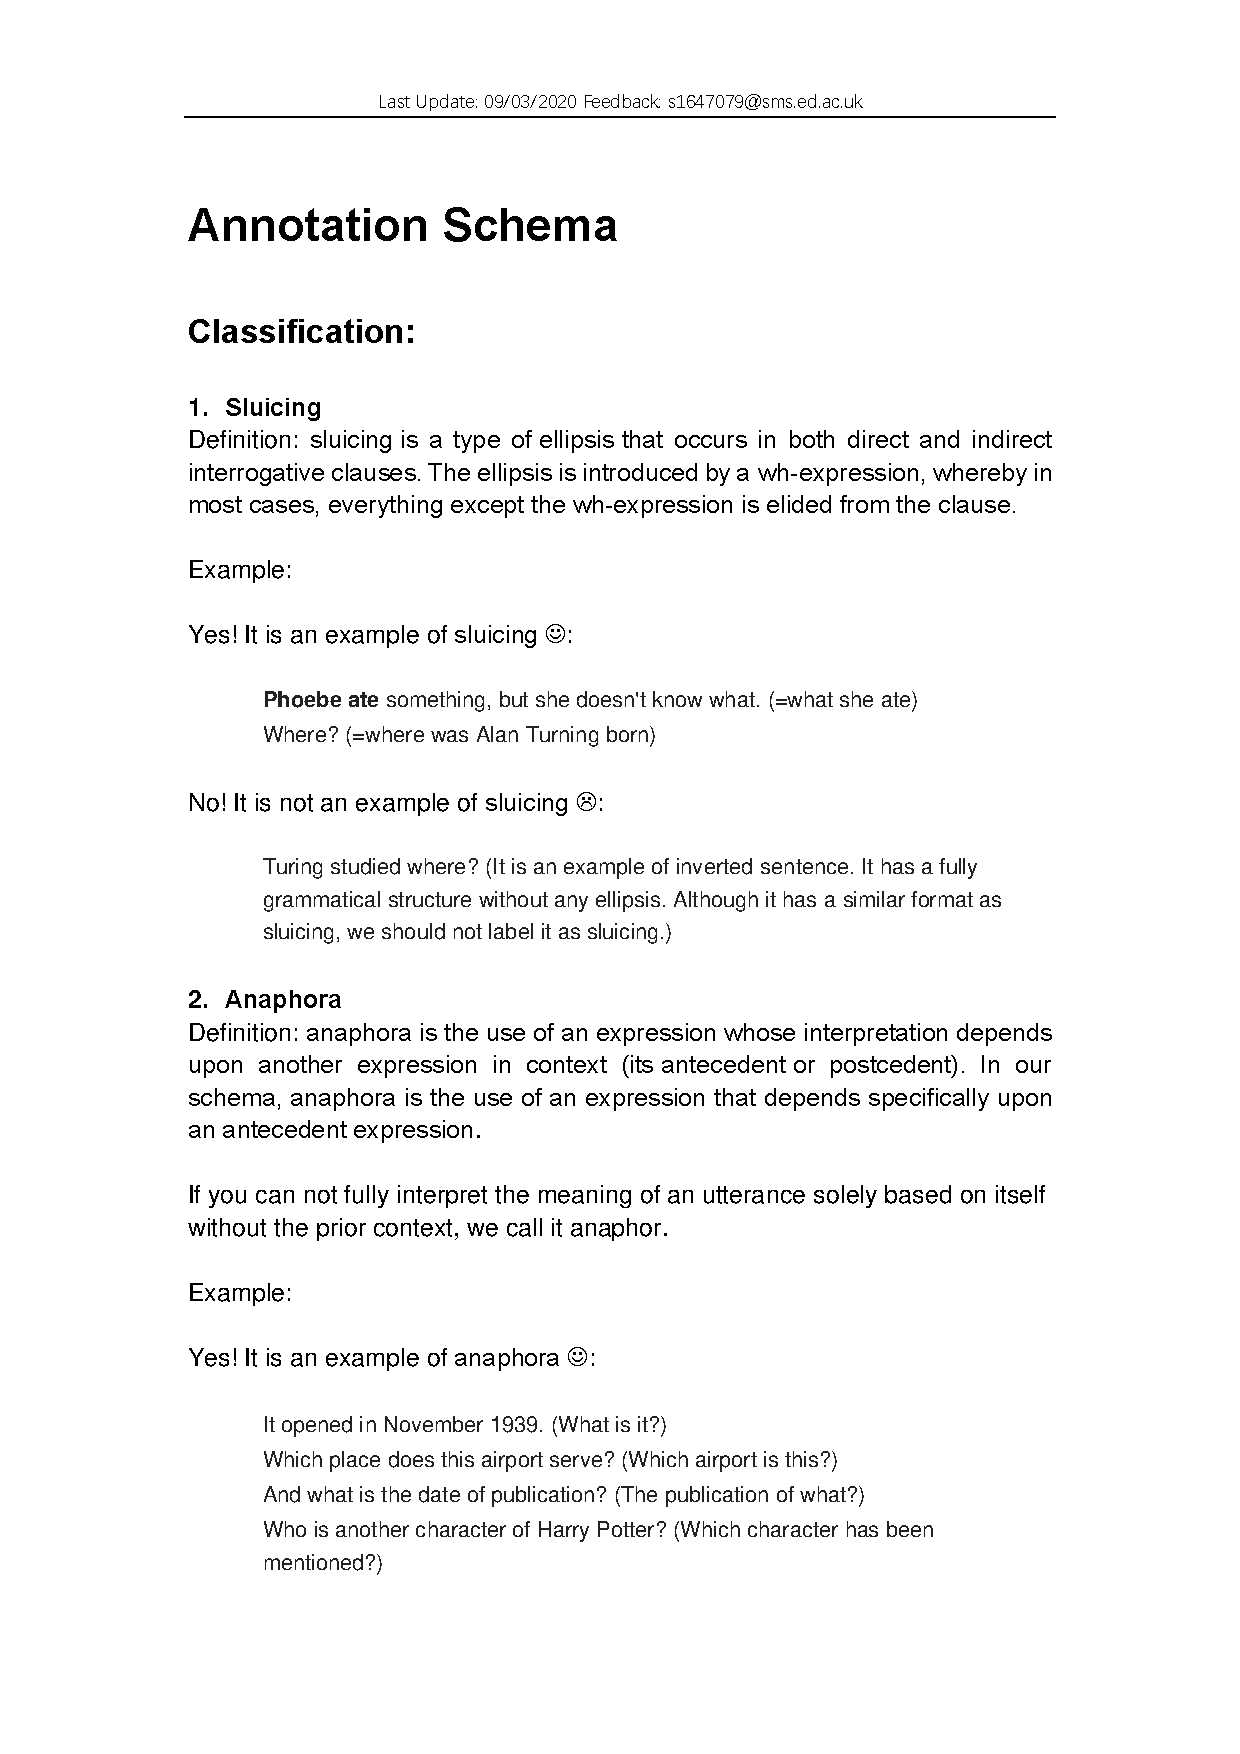
\includepdf[pages={1-}]{AnnotationSchema.pdf}
\label{appendix:annotation}

\chapter{Questionnaire Testing}


\end{document}